\documentclass[12pt,a4paper]{article}

\usepackage[margin=0.75in]{geometry}
\usepackage{xcolor}
\usepackage{amsmath,amssymb}
\usepackage{booktabs}
\usepackage{tabularx}
\usepackage{tcolorbox}
\usepackage{listings}
\usepackage{helvet}               
\usepackage[scaled=1.10]{inconsolata} 
\usepackage{graphicx}
\usepackage{subcaption}
\usepackage{float}
\usepackage{tikz}
\usepackage{hyperref}
\usepackage{booktabs} 
\usepackage{siunitx}  
\usetikzlibrary{positioning, arrows.meta, calc}

\hypersetup{
    colorlinks=true,
    urlcolor=blue
}

% Color definitions
\definecolor{codegreen}{rgb}{0,0.6,0}
\definecolor{codegray}{rgb}{0.5,0.5,0.5}
\definecolor{codepurple}{rgb}{0.58,0,0.82}
\definecolor{codeblue}{rgb}{0.13,0.29,0.53}
\definecolor{backcolour}{rgb}{0.96,0.96,0.96}

% Shared base style configuration
\lstset{
    backgroundcolor=\color{backcolour},   
    basicstyle=\ttfamily\footnotesize,
    breakatwhitespace=false,         
    breaklines=true,                 
    captionpos=b,                    
    keepspaces=true,                 
    numbers=left,                    
    numbersep=5pt,                   
    numberstyle=\tiny\color{codegray},
    showspaces=false,                
    showstringspaces=false,
    showtabs=false,                  
    tabsize=4
}

% Style definition for Python
\lstdefinestyle{pystyle}{
    language=Python,
    commentstyle=\color{codegreen},
    keywordstyle=\color{magenta},
    stringstyle=\color{codepurple}
}

% Style definition for C++
\lstdefinestyle{cppstyle}{
    language=C++,
    commentstyle=\color{codegreen},
    keywordstyle=\color{codeblue}\bfseries,
    stringstyle=\color{codepurple},
    morekeywords={std, cout, endl, vector}
}

\lstset{
    breaklines=true,
    breakatwhitespace=false,
    literate={,}{,{\penalty0}}{1} {.}{.{\penalty0}}{1}
}

\title{Digital Thermometer}
\author{
  \textbf{Arjun R Iyengar} \\
  \small EE26BTECH11202
  \and
  \textbf{Arya Sudhirkumar Neel} \\
  \small EE26BTECH11203
  \and
  \textbf{Tejas L.P} \\
  \small EE26BTECH11231 \\ \\}
\date{October 2026}

\begin{document}
\maketitle

\section*{Day 1}
\noindent{We spent this day understanding the components, the circuit, and the connections required to be made. To account for the lack of an external ADC, we decided to use a voltage divider circuit with the Arduino's built-in ADC.}

\section*{Day 2}
\noindent{We started building the circuit using the Arduino's built-in ADC and a voltage divider circuit. However, when we uploaded temporary code to display the temperature, the LCD displayed nothing at all---only the backlight was lit. When we turned the knob of the potentiometer, a few dark lines appeared, but the temperature was never displayed.} \\ \\

\noindent{We didn't know which component was causing the issue, so we decided to test the LCD first. We made simple connections just to check if the LCD could display ``HELLO WORLD'' as seen in Figure~\ref{fig:faulty_lcd}. We uploaded the code and found the same issue again: only the backlight lit up, but nothing was actually displayed. We observed the same few dark lines appearing momentarily when we turned the knob of the potentiometer.} \\

\begin{figure}[H]
    \centering
    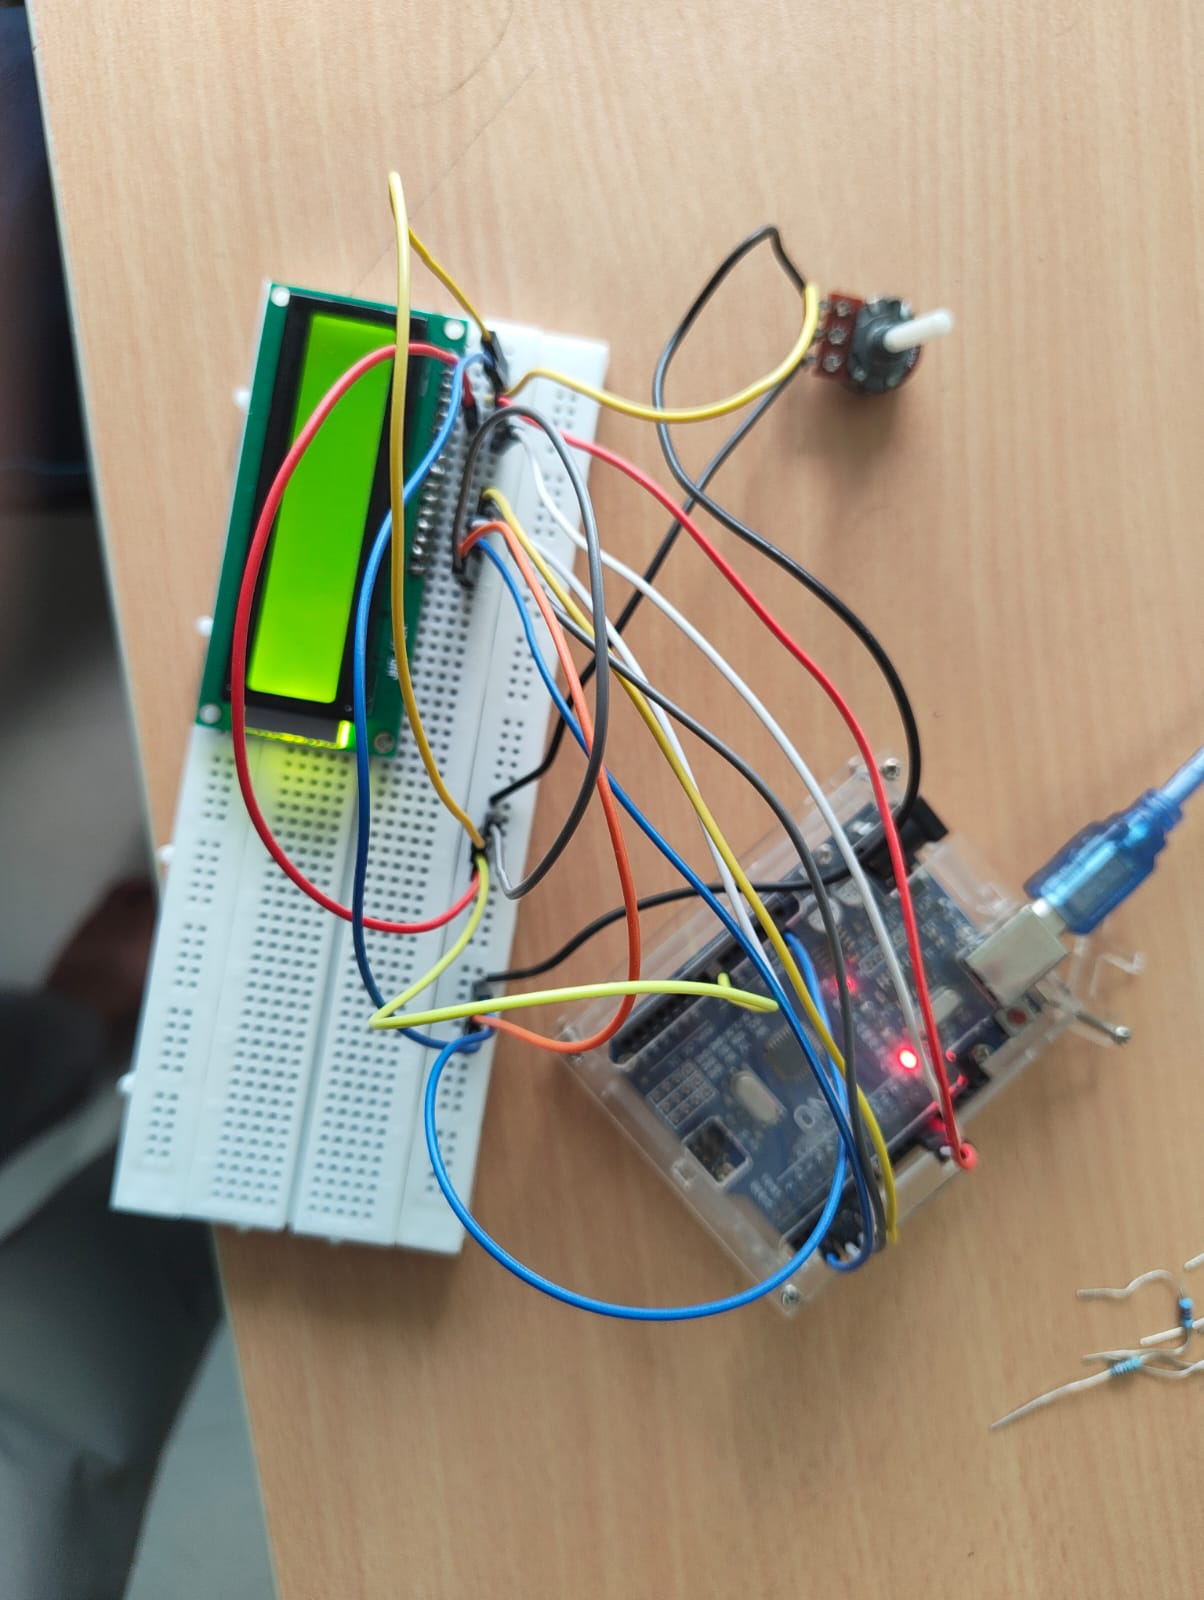
\includegraphics[width=0.5\linewidth]{figs/faulty_lcd.jpeg}
    \caption{Faulty LCD}
    \label{fig:faulty_lcd}
\end{figure}

\noindent{We now knew that the potentiometer was working and needed to isolate the error. There could have been various issues, such as faulty breadboard rails; however, that was unlikely since we had used the same breadboard to test previous circuits. The first intuitive step was to replace the LCD display. We borrowed another display from a friend and tested it out. It turned out that the original display was indeed faulty, as the new display worked correctly.}

\begin{figure}[H]
    \centering
    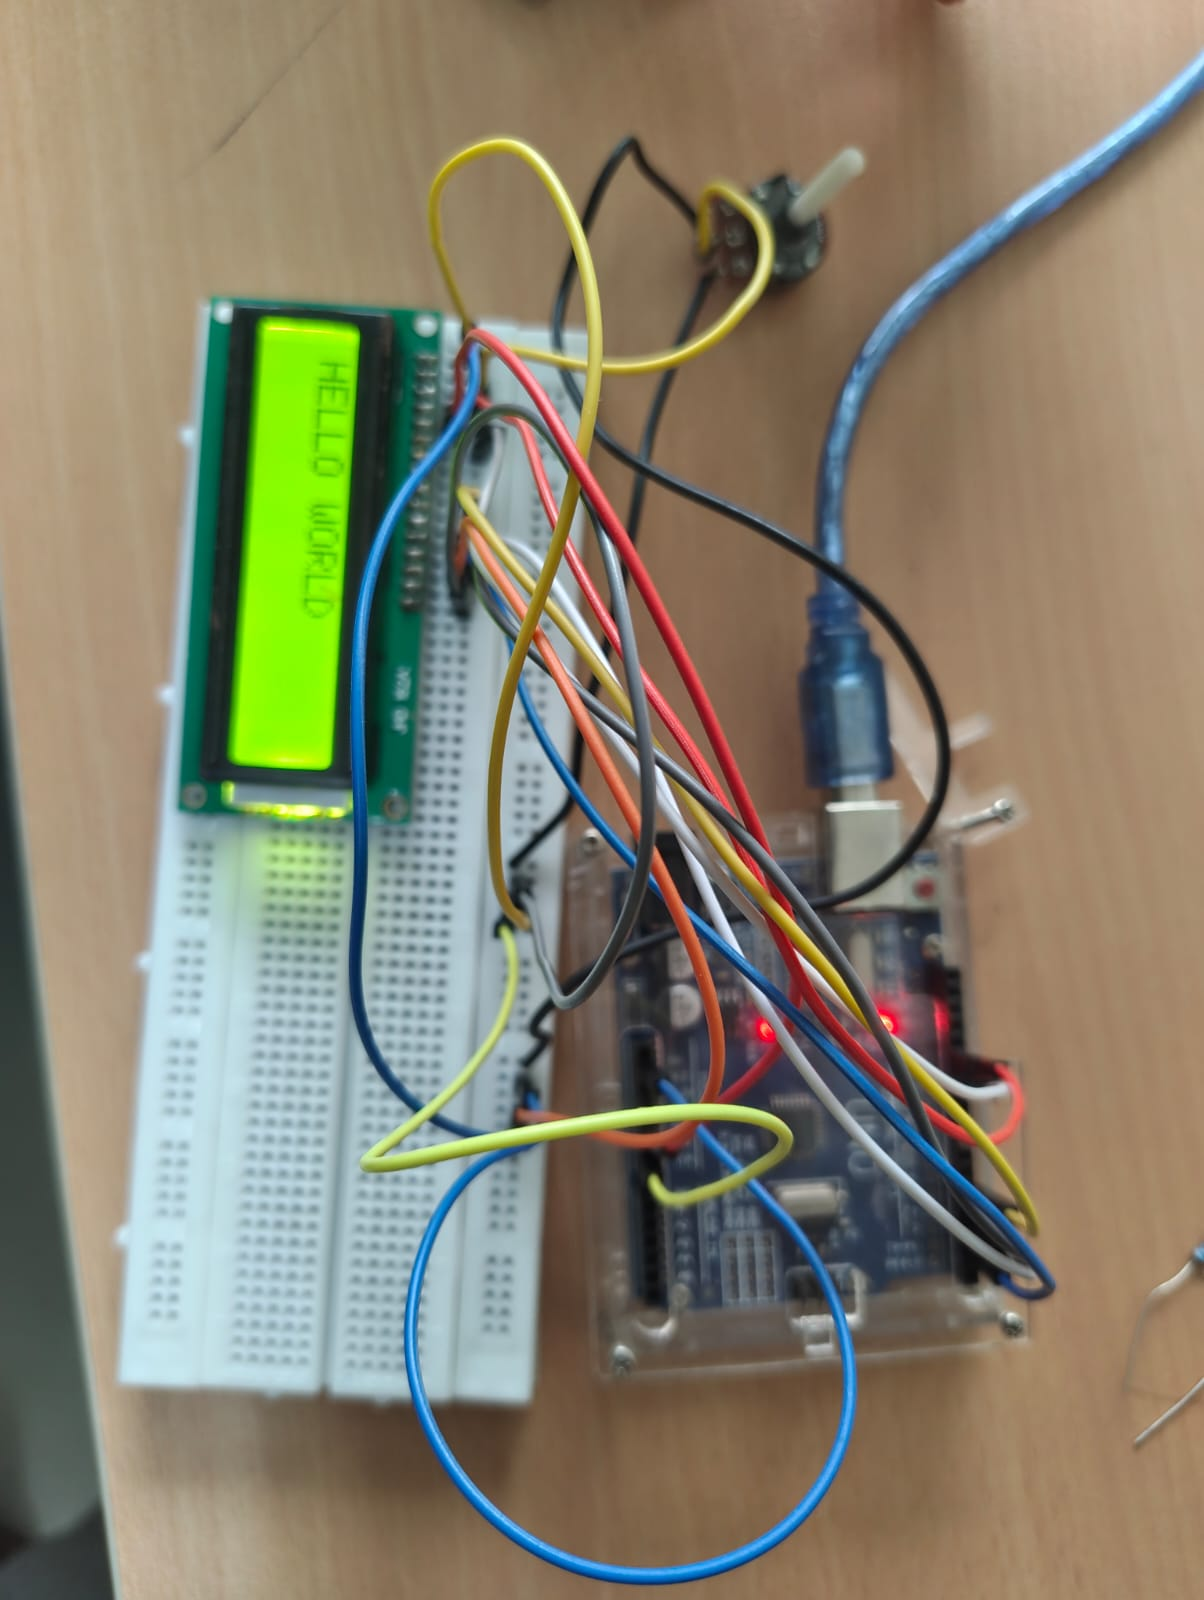
\includegraphics[width=0.5\linewidth]{figs/Corrected_lcd.jpeg}
    \caption{``HELLO WORLD'' displayed successfully}
    \label{fig:corrected_lcd}
\end{figure}

\section*{Day 3}
\noindent{Now, we could move ahead and verify if the thermometer showed valid readings. We measured the resistance of the reference resistor ($119\,\Omega$) and the supply rail ($V_{\text{cc}} = 5.08\,\text{V}$) using a multimeter. We implemented a simple test script without the LSQ model to check baseline readings. However, as expected, there was a deviation of around $5^\circ\text{C}$. This confirmed that our hardware was functioning correctly and that we needed to apply the LSQ model to minimize measurement error. The test code used was:}

\begin{lstlisting}[style=cppstyle]
#include <LiquidCrystal.h>

LiquidCrystal lcd(12, 11, 5, 4, 3, 2);

const int sensorPin = A0;
const float Vcc = 5.08;        // Measured supply rail voltage
const float R_fixed = 119.0;   // Measured reference resistor

void setup() {
  lcd.begin(16, 2);
}

void loop() {
  // 1. Oversample 16 readings
  long adcSum = 0;
  for (int i = 0; i < 16; i++) {
    adcSum += analogRead(sensorPin);
    delay(2);
  }
  float avgADC = (float)adcSum / 16.0;

  // 2. Voltage across PT100
  float X = avgADC * (Vcc / 1023.0);

  // 3. Calculated PT100 resistance: R_pt = R_fixed * (X / (Vcc - X))
  float R_pt = R_fixed * (X / (Vcc - X));

  // 4. Standard PT100 conversion (approx 0.3851 Ohms per degree Celsius)
  float tempC = (R_pt - 100.0) / 0.3851;

  // 5. Display Voltage and Resistance on line 1, Temp on line 2
  lcd.setCursor(0, 0);
  lcd.print("V:");
  lcd.print(X, 2);
  lcd.print("V R:");
  lcd.print(R_pt, 1);
  lcd.print((char)244); // Ohm symbol

  lcd.setCursor(0, 1);
  lcd.print("Temp: ");
  lcd.print(tempC, 1);
  lcd.print(" ");
  lcd.write(223);
  lcd.print("C   ");

  delay(400);
}
\end{lstlisting}

\noindent{The resulting initial outputs were recorded as follows:}

\begin{figure}[H]
    \centering
    \begin{subfigure}{0.45\textwidth}
        \centering
        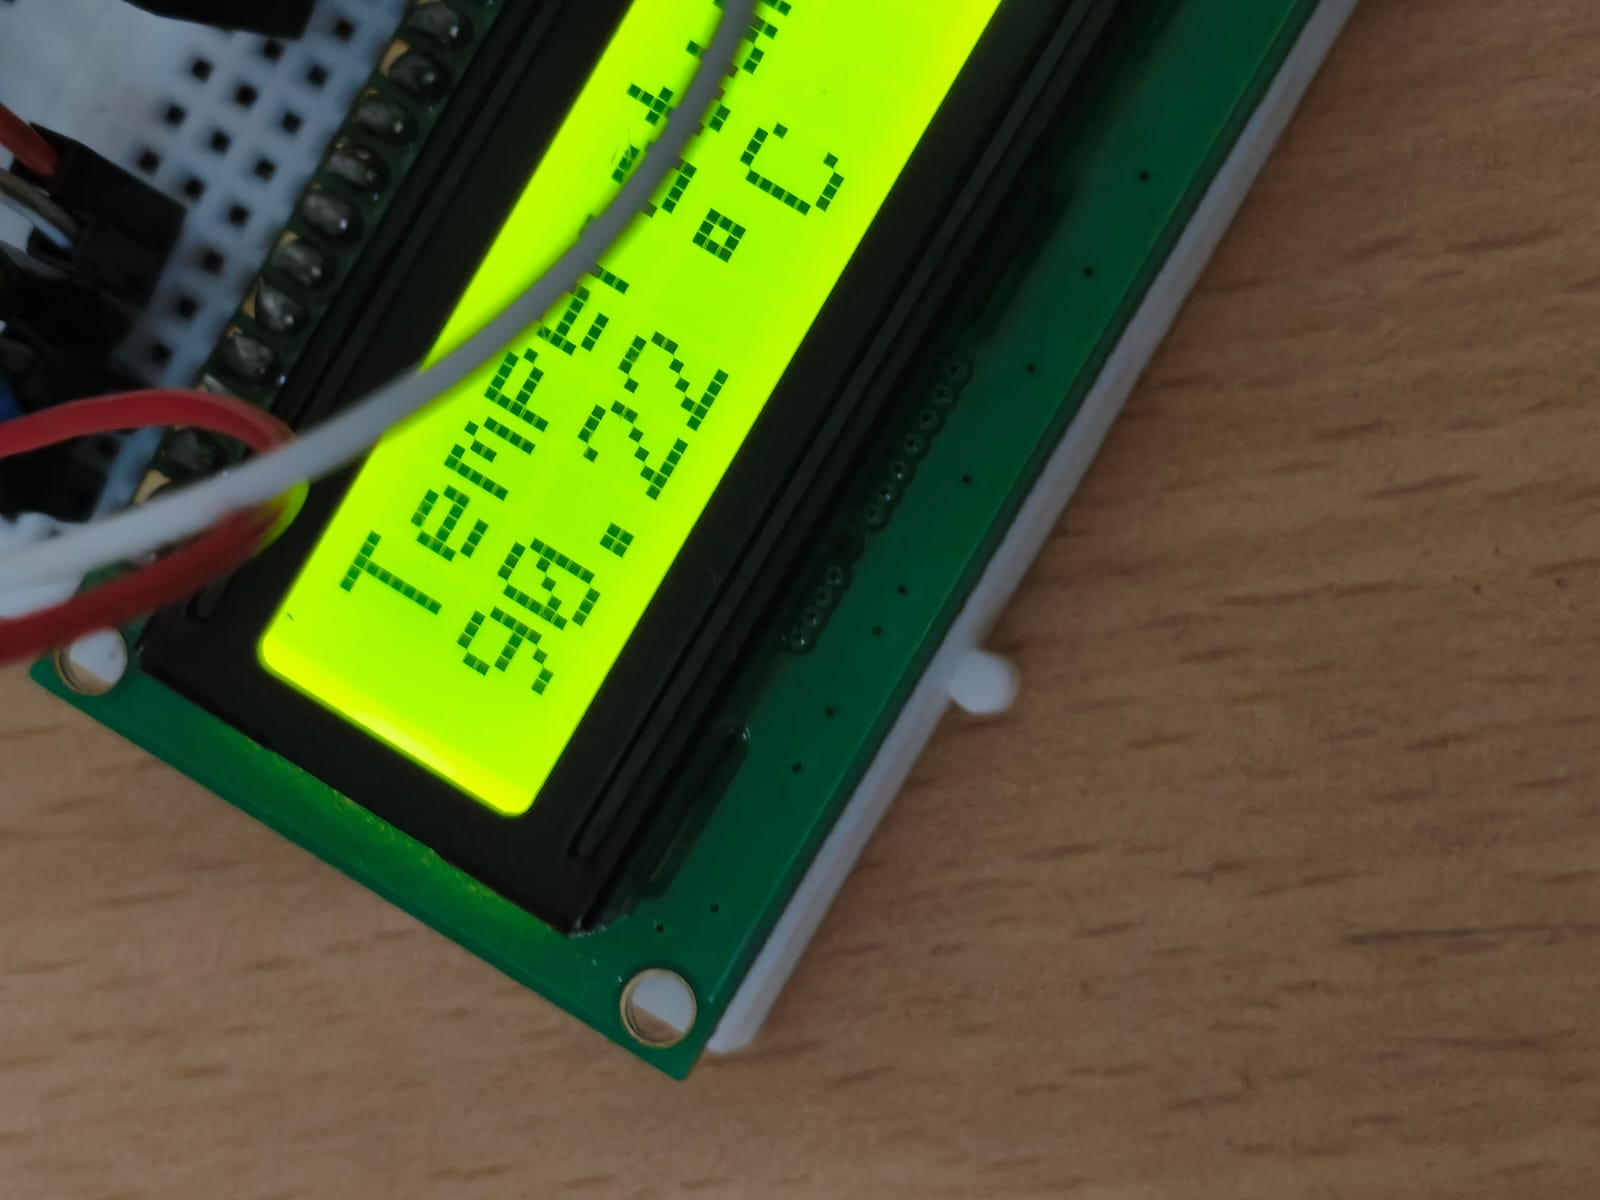
\includegraphics[width=\textwidth, height=10cm, keepaspectratio]{figs/Breadboard_test.jpeg}
        \caption{Our reading}
    \end{subfigure}
    \hfill
    \begin{subfigure}{0.45\textwidth}
        \centering
        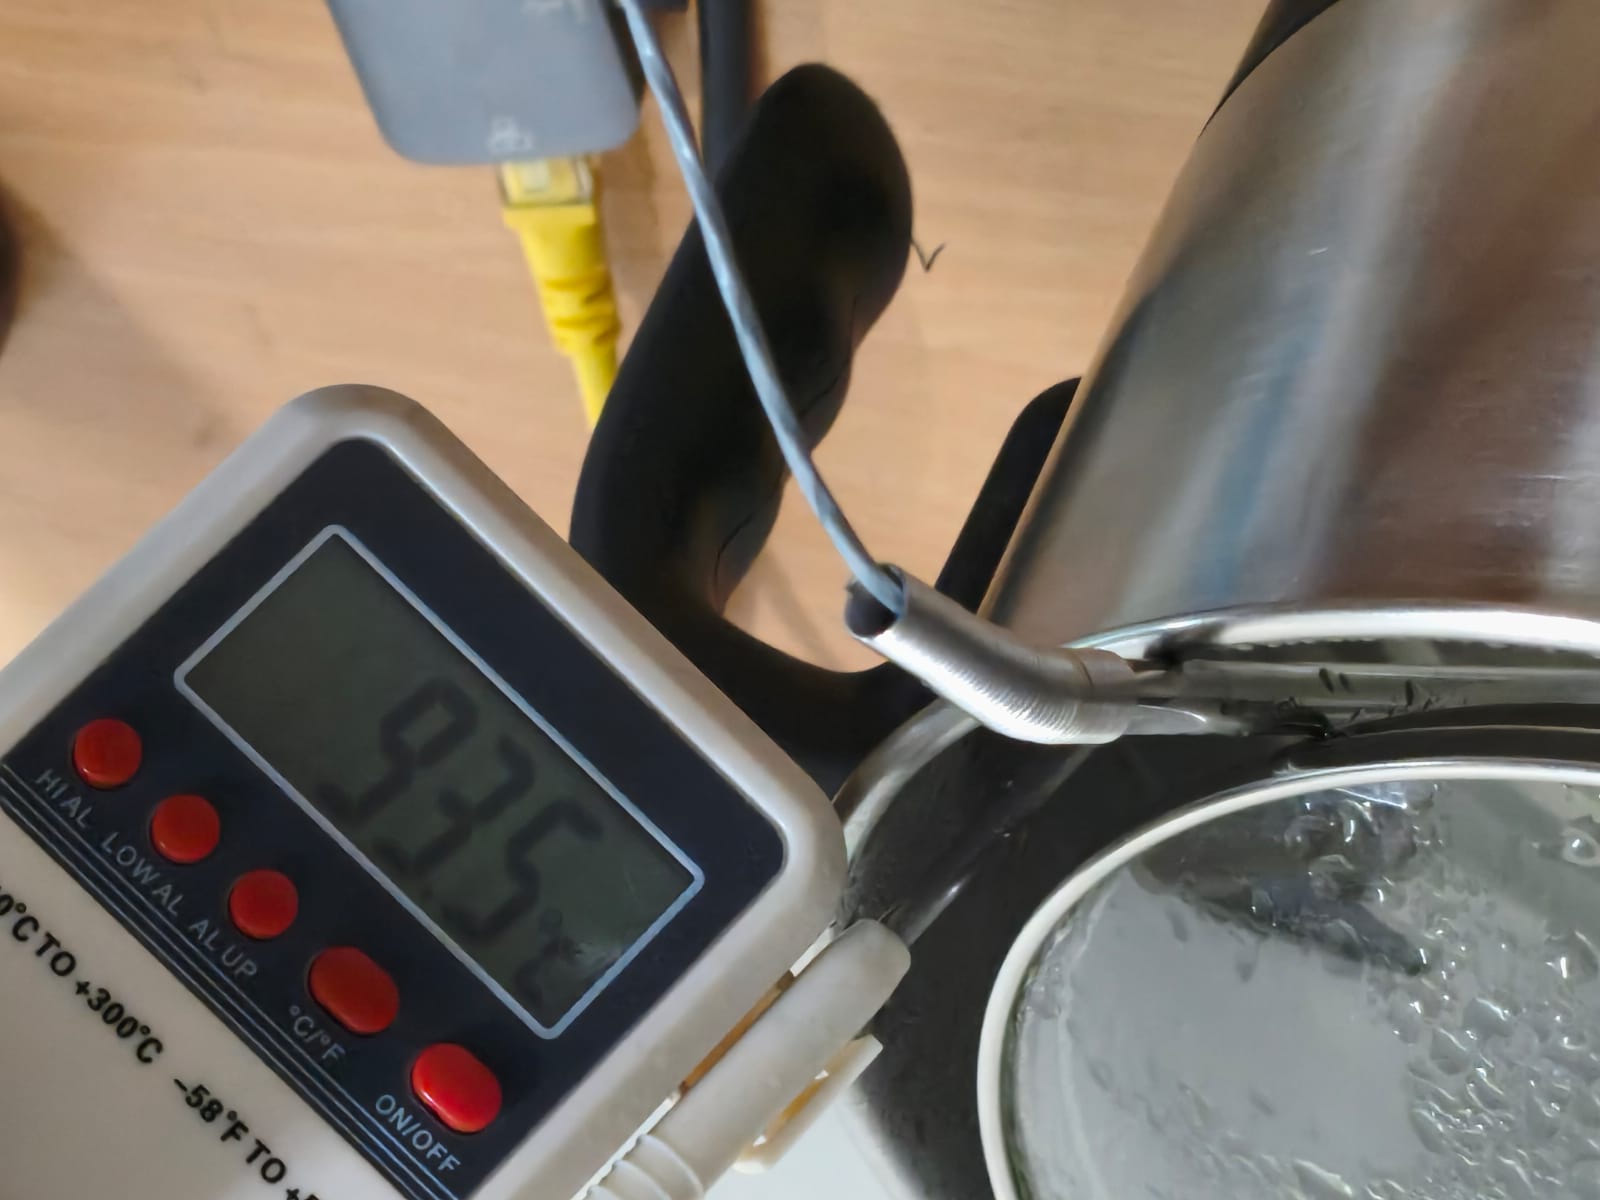
\includegraphics[width=\textwidth, height=8cm, keepaspectratio]{figs/Breadboard-Test_1.jpeg}
        \caption{Actual reference reading}
    \end{subfigure}
\end{figure}

\noindent{Before proceeding to final calibration, we soldered the circuit onto a perfboard. This required careful layout planning to account for enclosure space and component heights. The soldering process took approximately 5 hours. The assembled board is shown below:}

\begin{figure}[H]
    \centering
    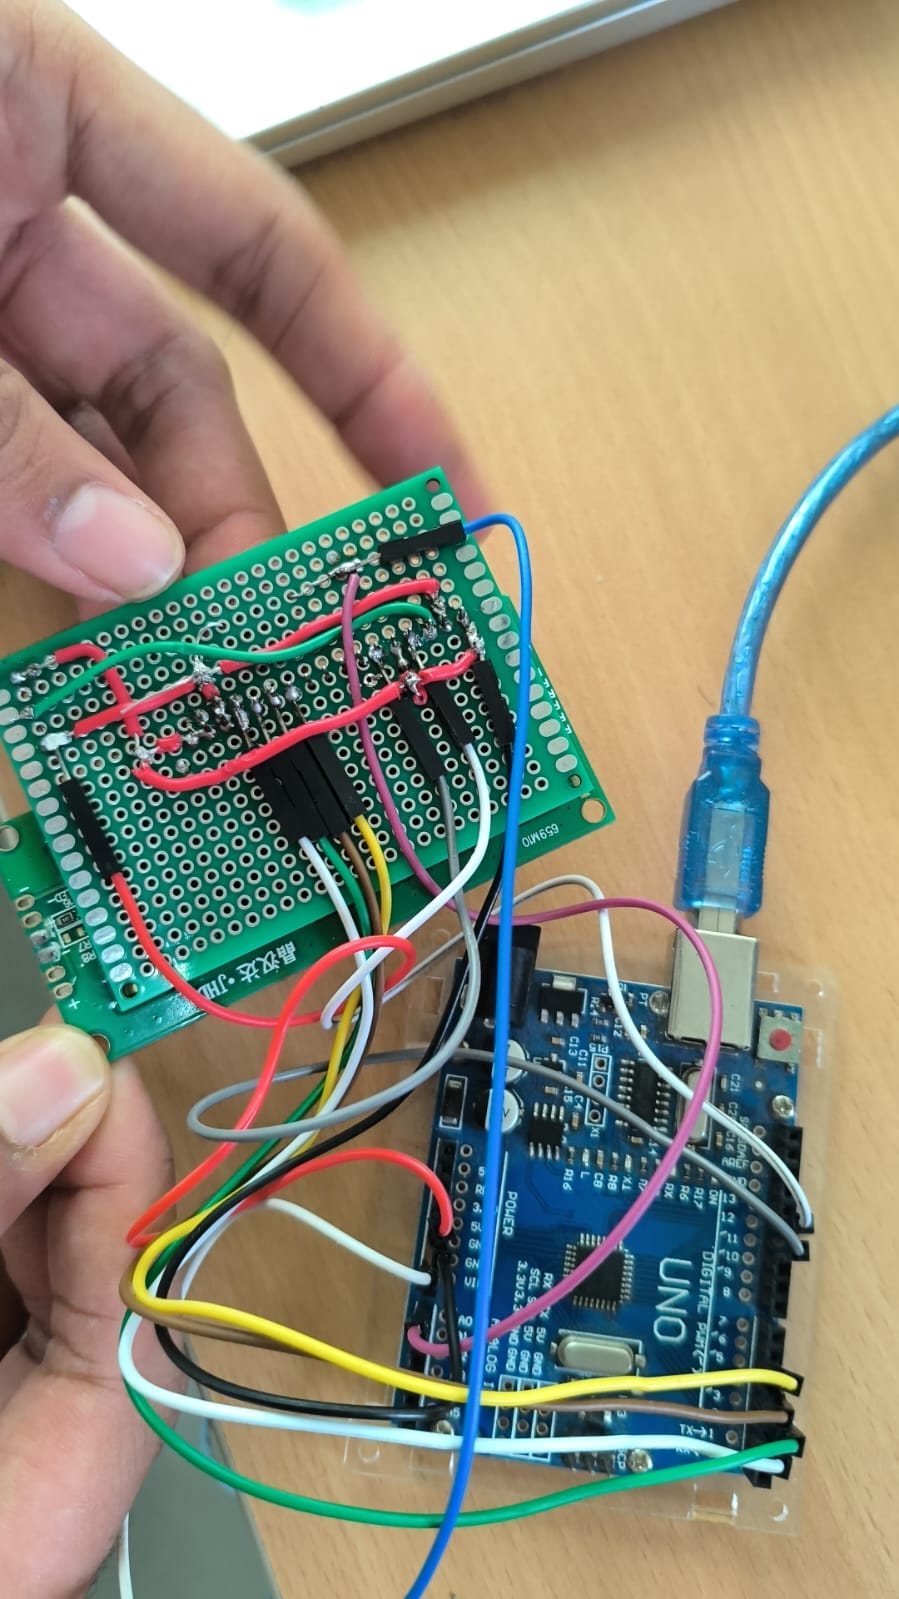
\includegraphics[width=0.5\linewidth]{figs/Soldering.jpeg}
    \caption{Soldered PCB assembly}
\end{figure}

\section*{Days 4 and 5 - Finding the Right Model}
\noindent{We next attempted to implement the paper's inverse LSQ model with the voltage divider, modifying the coefficients to account for our different reference resistance. However, this approach failed; the room temperature reading alone was offset by approximately $4.5^\circ\text{C}$.}

\begin{figure}[H]
\centering
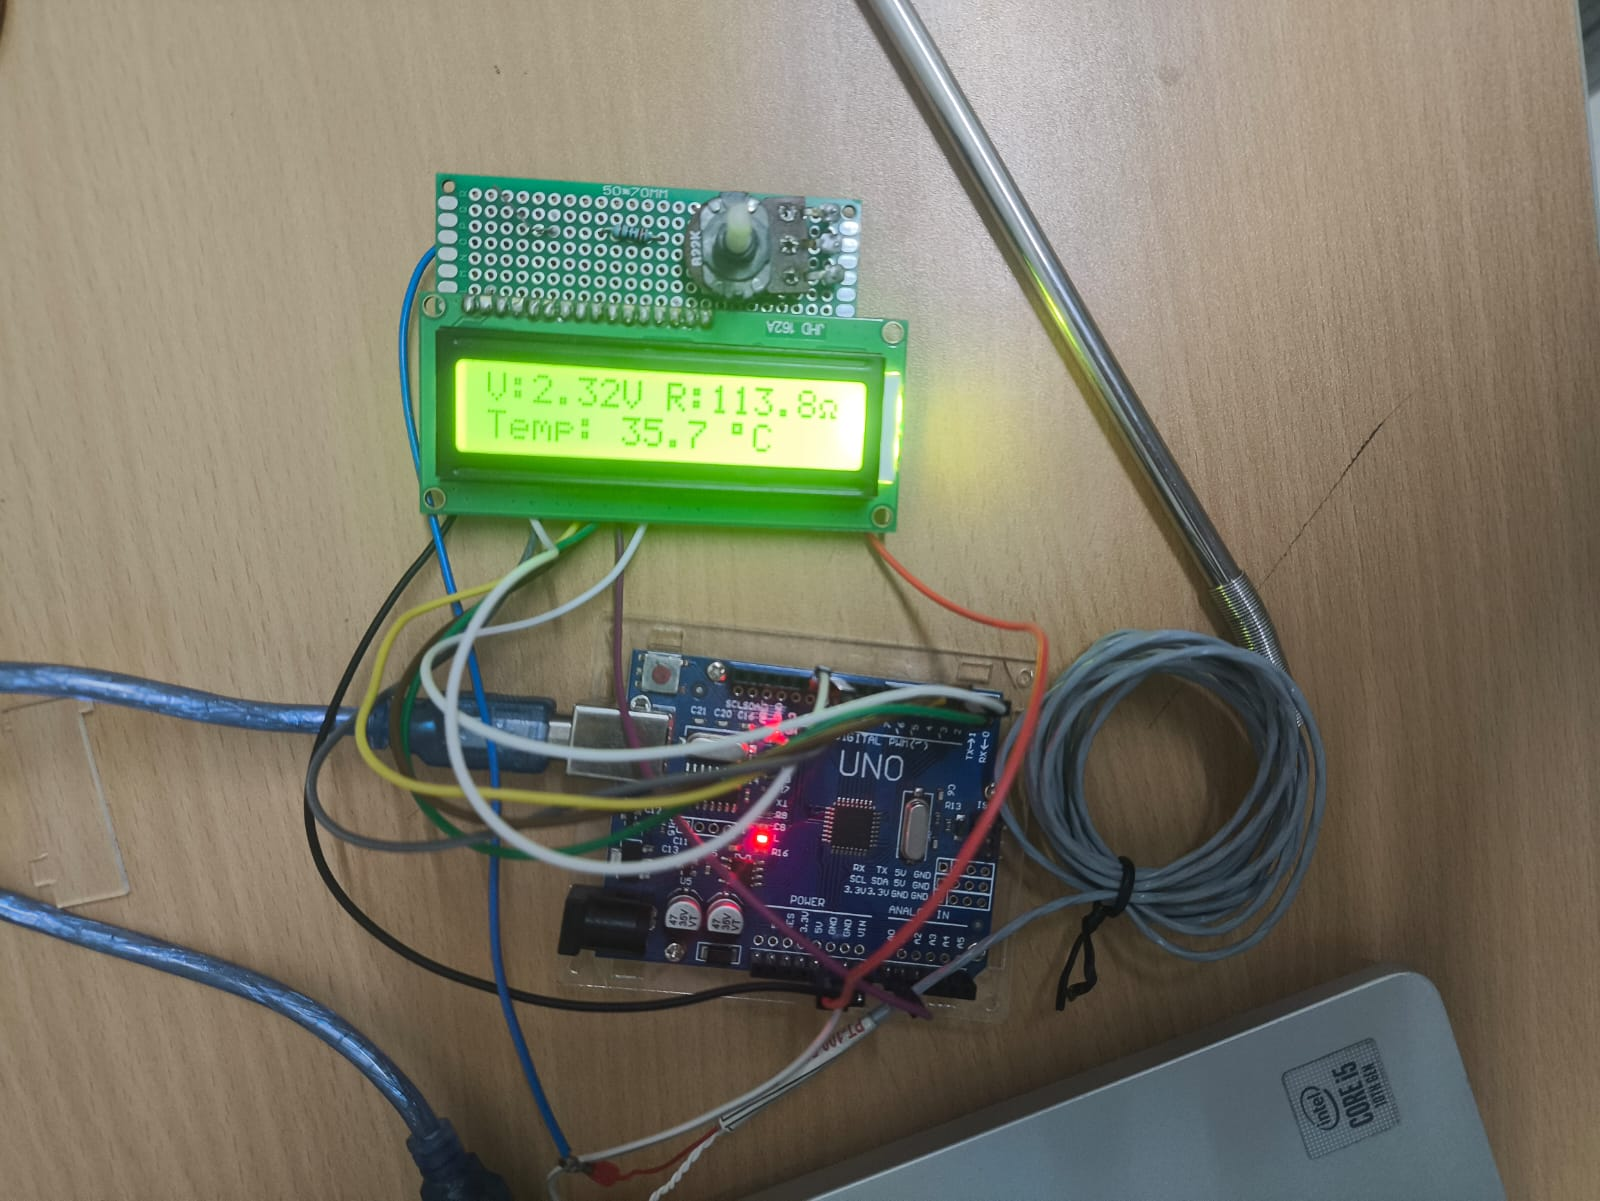
\includegraphics[width=\textwidth, height=10cm, keepaspectratio]{figs/Inverse-Wrong_reading.jpeg}
\caption{Erroneous inverse model reading at room temperature}
\end{figure}

\noindent{This meant we needed to calibrate the setup empirically and derive custom LSQ coefficients. Rather than taking only 3 data points to solve a system of equations, we opted to gather an overdetermined dataset across multiple temperatures and perform a quadratic least squares curve fit using NumPy's \texttt{polyfit} function.} \\

\begin{figure}[H]
    \centering
    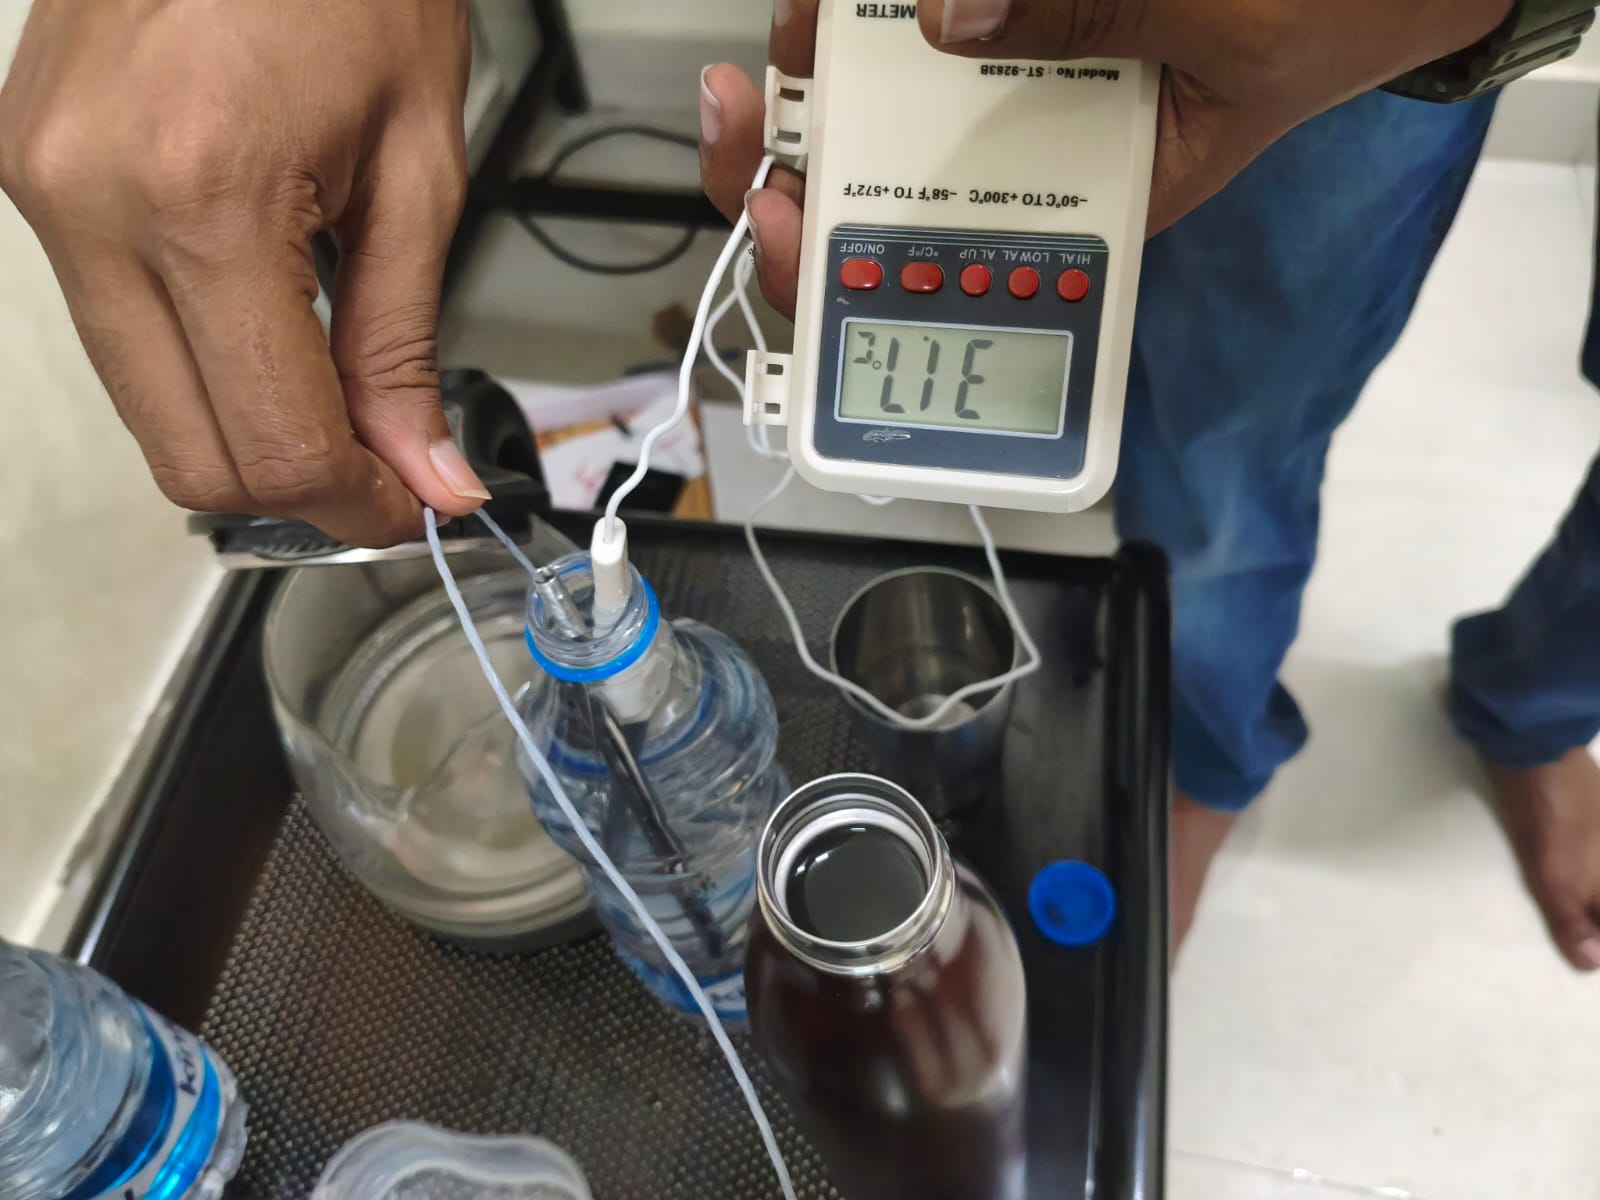
\includegraphics[width=0.5\linewidth]{figs/Calibration.jpeg}
    \caption{Calibration setup in progress}
\end{figure}

\noindent{We began calibration by heating water to boiling point and recording data continuously as it cooled, adding cold water to obtain $10^\circ\text{C}$ step intervals down to room temperature and below. Throughout the process, the PT100 probe was fully submerged and stirred continuously to ensure uniform temperature and avoid thermal drift errors. Our initial run yielded 7 samples. Upon evaluating the resulting polynomial fit, we observed:}

\begin{itemize}
    \item Readings between $30^\circ\text{C}$ and $50^\circ\text{C}$ were relatively accurate, with marginal errors of $2$--$3^\circ\text{C}$.
    \item Readings at higher temperatures were significantly off, showing errors up to $7^\circ\text{C}$.
    \item Sub-ambient readings were inaccurate due to sparse data coverage at low temperatures.
\end{itemize}

\noindent{To address this, we expanded our dataset across the full temperature range, gathering a total of 14 points to improve fit stability. However, a loose wire connection forced us to resolder several joints, requiring a fresh calibration run, which was quite frustrating. The final verified calibration dataset is presented in Table~\ref{tab:pt100_calibration}:}

\begin{table}[H]
  \centering
  \caption{Empirical Calibration Data for PT100 Voltage Divider Circuit ($V_{cc} = 5.05\,\text{V}$)}
  \label{tab:pt100_calibration}
  \begin{tabular}{ccc}
    \toprule
    \textbf{Sample Point} & \textbf{Measured Voltage ($V$) [V]} & \textbf{Reference Temp ($T$) [$^\circ$C]} \\
    \midrule
    1  & 2.731183 & 95.3 \\
    2  & 2.701388 & 88.8 \\
    3  & 2.671593 & 77.9 \\
    4  & 2.646764 & 71.1 \\
    5  & 2.621935 & 66.3 \\
    6  & 2.602072 & 61.1 \\
    7  & 2.587175 & 55.5 \\
    8  & 2.567312 & 50.5 \\
    9  & 2.542483 & 44.3 \\
    10 & 2.527585 & 40.3 \\
    11 & 2.502757 & 35.9 \\
    12 & 2.487859 & 32.1 \\
    13 & 2.458065 & 26.3 \\
    14 & 2.438201 & 21.8 \\
    \bottomrule
  \end{tabular}
\end{table}

\noindent{The Python script used to compute the polynomial coefficients is given below:}

\begin{lstlisting}[style=pystyle]
import numpy as np

# V and T readings (measured voltage V, reference temperature T)
V = np.array([2.731183, 2.701388, 2.671593, 2.646764, 2.621935, 2.602072, 2.587175, 2.567312, 2.542483, 2.527585, 2.502757, 2.487859, 2.458065, 2.438201])
T = np.array([95.3, 88.8, 77.9, 71.1, 66.3, 61.1, 55.5, 50.5, 44.3, 40.3, 35.9, 32.1, 26.3, 21.8])

# Least squares polynomial fit of degree 2 (quadratic: T = a*V^2 + b*V + c)
coefficients = np.polyfit(V, T, 2)

a = coefficients[0]
b = coefficients[1]
c = coefficients[2]

print("Quadratic coefficients:")
print(f"a (V^2): {a:.8f}")
print(f"b (V):   {b:.8f}")
print(f"c (Intercept): {c:.8f}")
print(f"Fitted Equation: T = {a:.4f} * V^2 + {b:.4f} * V + {c:.4f}")
\end{lstlisting}

\noindent{Executing the regression script yielded the following coefficients:}
\begin{align*}
    a &= 170.62478693 \\
    b &= -627.58944219 \\
    c &= 537.54348189
\end{align*}

\noindent{The figures below demonstrate the real-world performance of the calibrated thermometer across different temperature regimes:}

\begin{figure}[H]
    \centering
    \begin{subfigure}{0.45\textwidth}
        \centering
        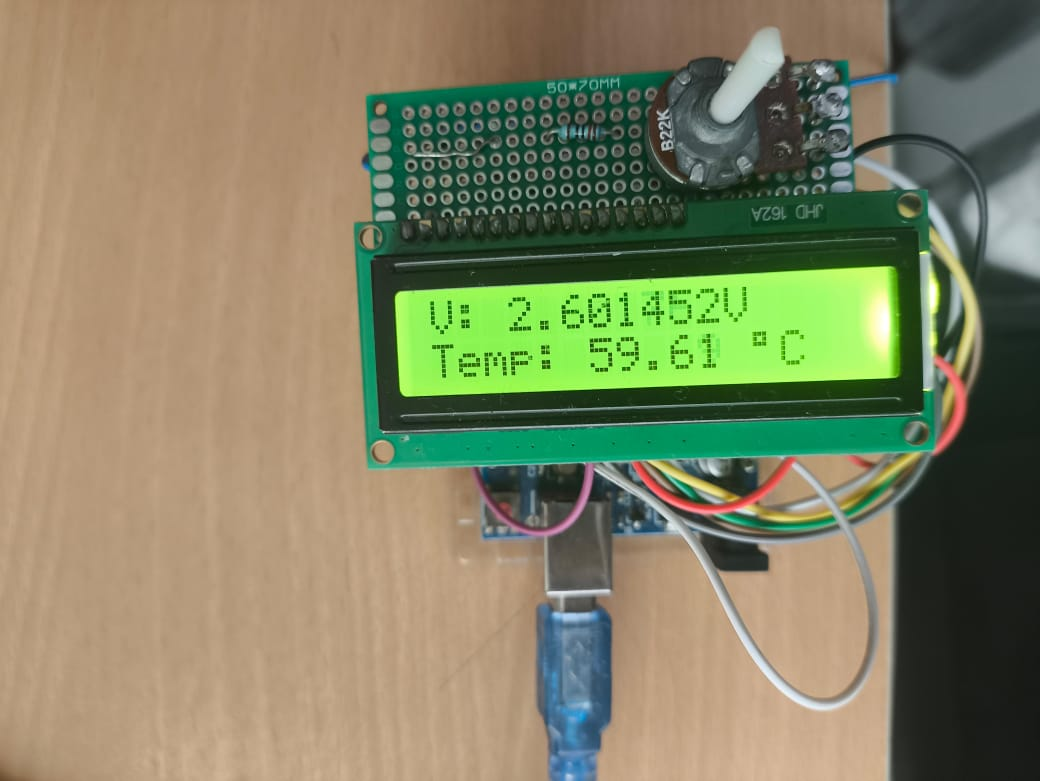
\includegraphics[width=\textwidth, height=10cm, keepaspectratio]{figs/Working-60.jpeg}
        \caption{Our reading ($60^\circ\text{C}$ range)}
    \end{subfigure}
    \hfill
    \begin{subfigure}{0.45\textwidth}
        \centering
        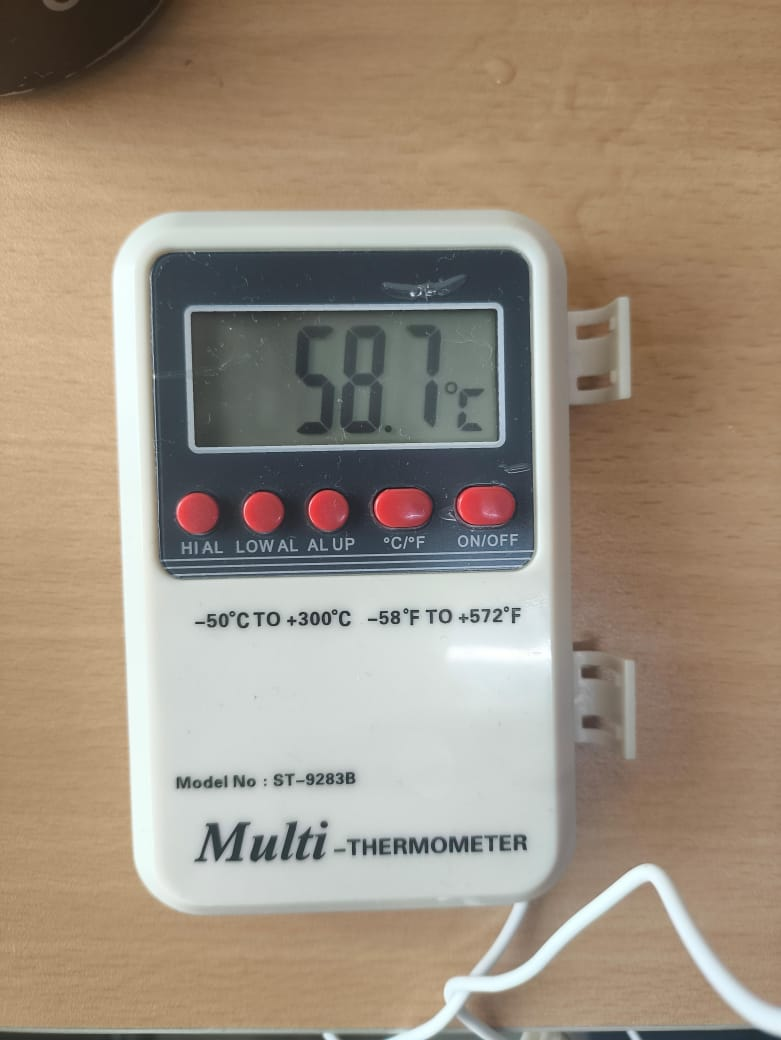
\includegraphics[width=\textwidth, height=10cm, keepaspectratio]{figs/Working-60_1.jpeg}
        \caption{Reference reading}
    \end{subfigure}
\end{figure}

\begin{figure}[H]
    \centering
    \begin{subfigure}{0.45\textwidth}
        \centering
        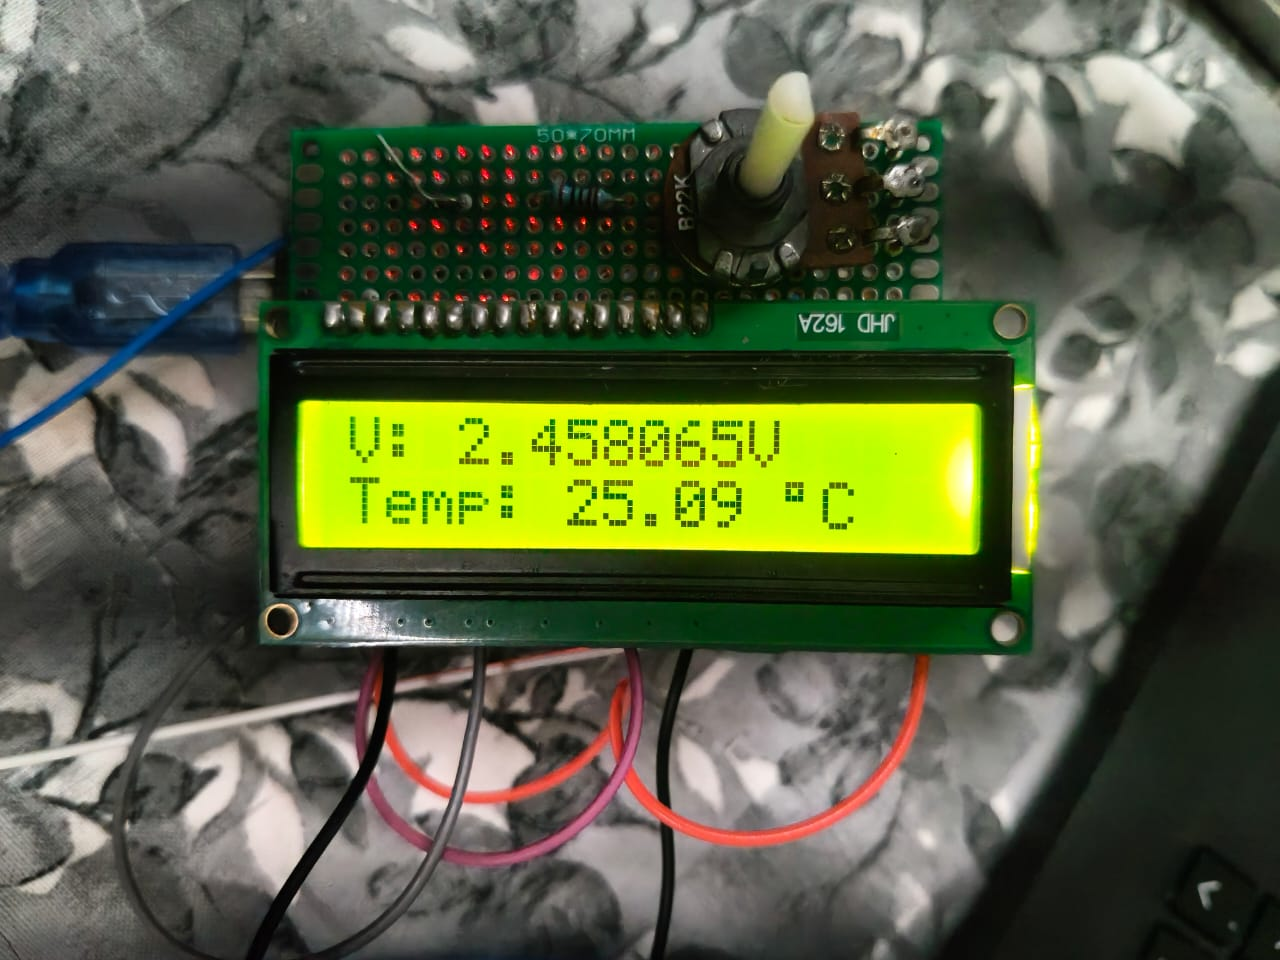
\includegraphics[width=\textwidth, height=10cm, keepaspectratio]{figs/Working-25.jpeg}
        \caption{Our reading ($25^\circ\text{C}$ range)}
    \end{subfigure}
    \hfill
    \begin{subfigure}{0.45\textwidth}
        \centering
        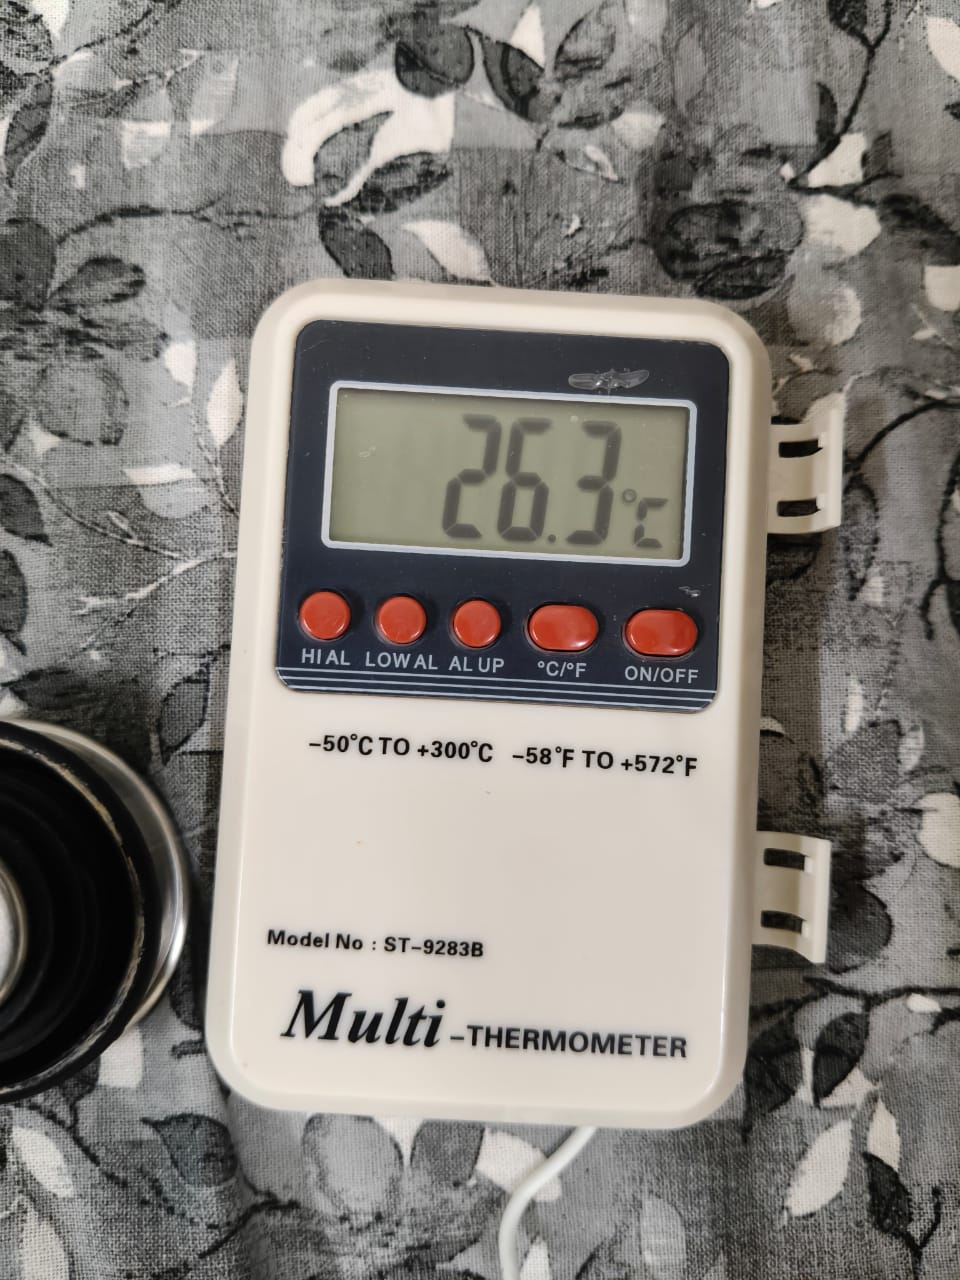
\includegraphics[width=\textwidth, height=8cm, keepaspectratio]{figs/Working-25_1.jpeg}
        \caption{Reference reading}
    \end{subfigure}
\end{figure}

\begin{figure}[H]
    \centering
    \begin{subfigure}{0.45\textwidth}
        \centering
        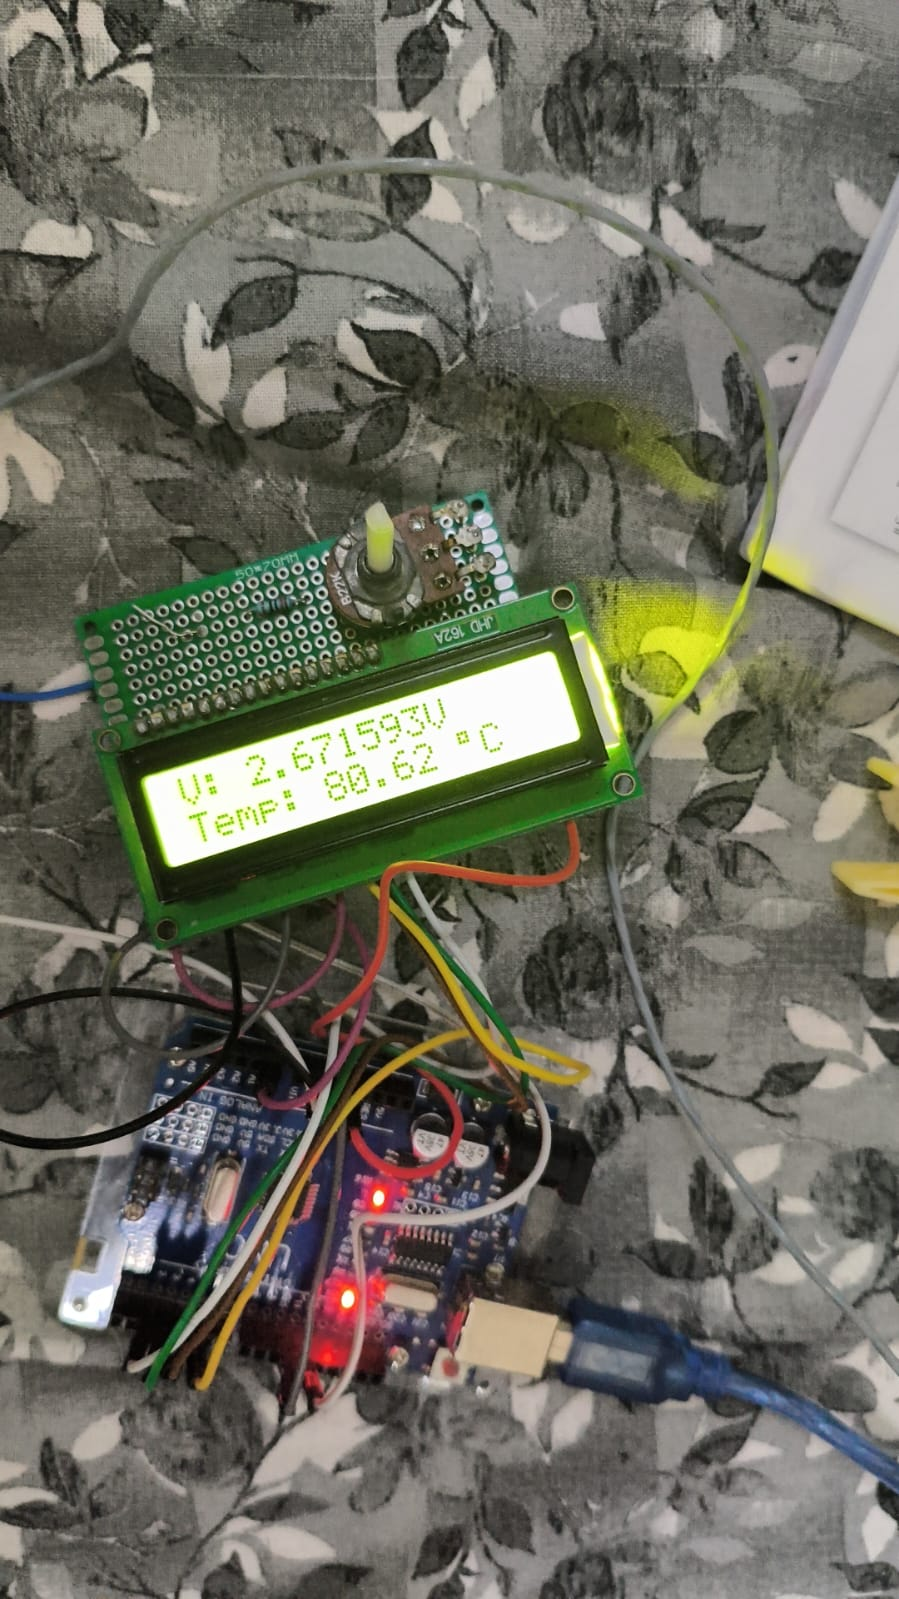
\includegraphics[width=\textwidth, height=10cm, keepaspectratio]{figs/Working-80.jpeg}
        \caption{Our reading ($80^\circ\text{C}$ range)}
    \end{subfigure}
    \hfill
    \begin{subfigure}{0.45\textwidth}
        \centering
        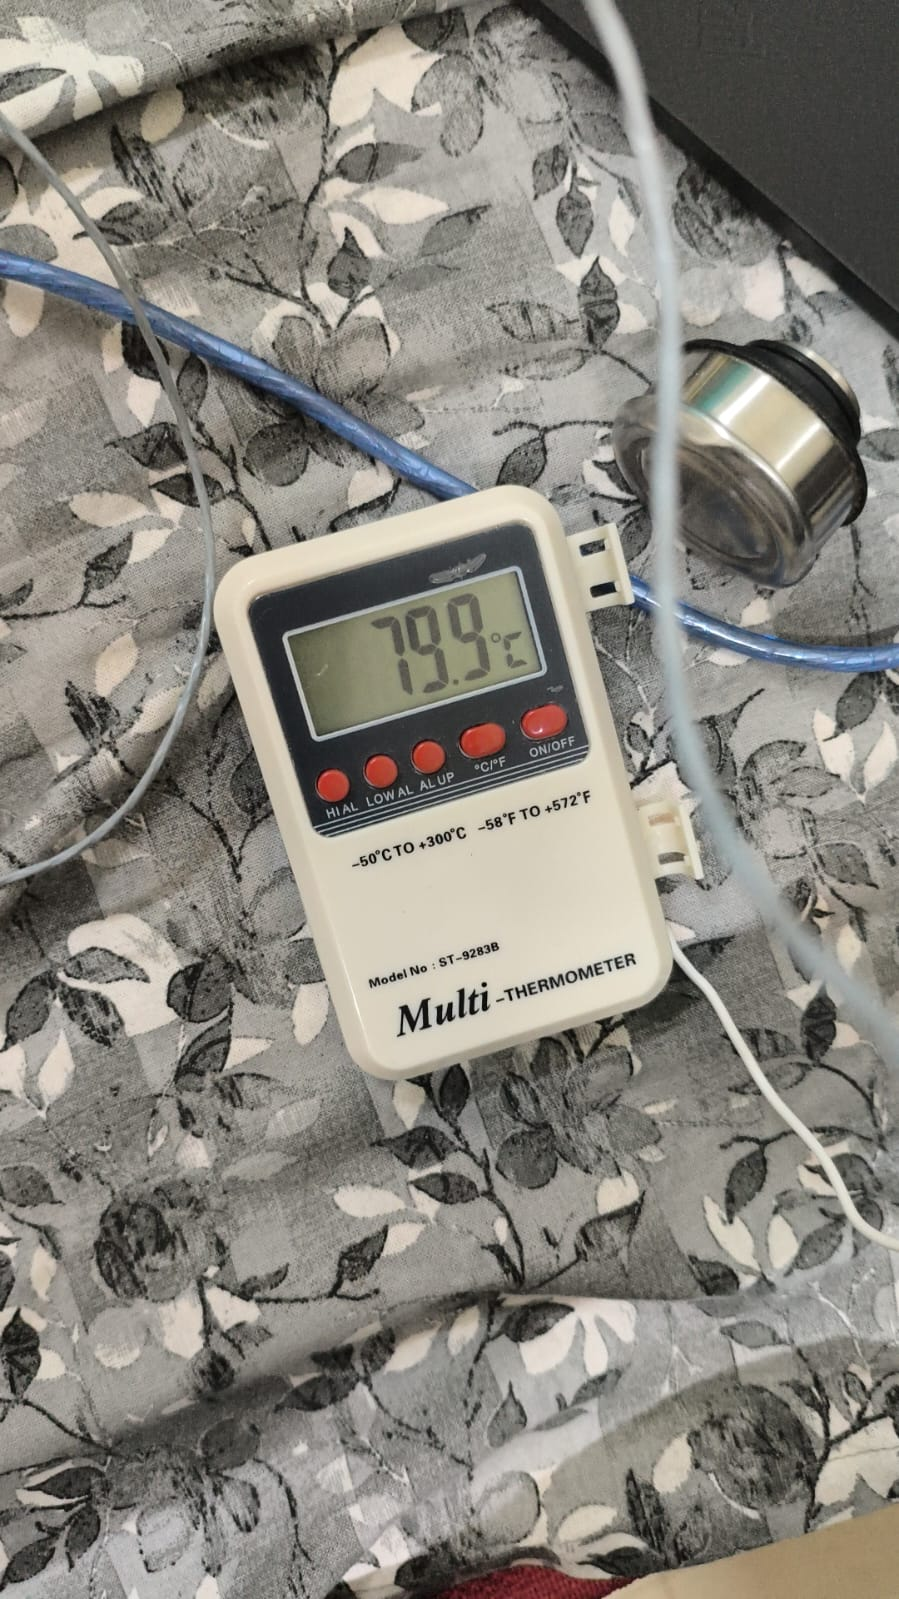
\includegraphics[width=\textwidth, height=10cm, keepaspectratio]{figs/Working-80_1.jpeg}
        \caption{Reference reading}
    \end{subfigure}
\end{figure}

\begin{figure}[H]
    \centering
    \begin{subfigure}{0.45\textwidth}
        \centering
        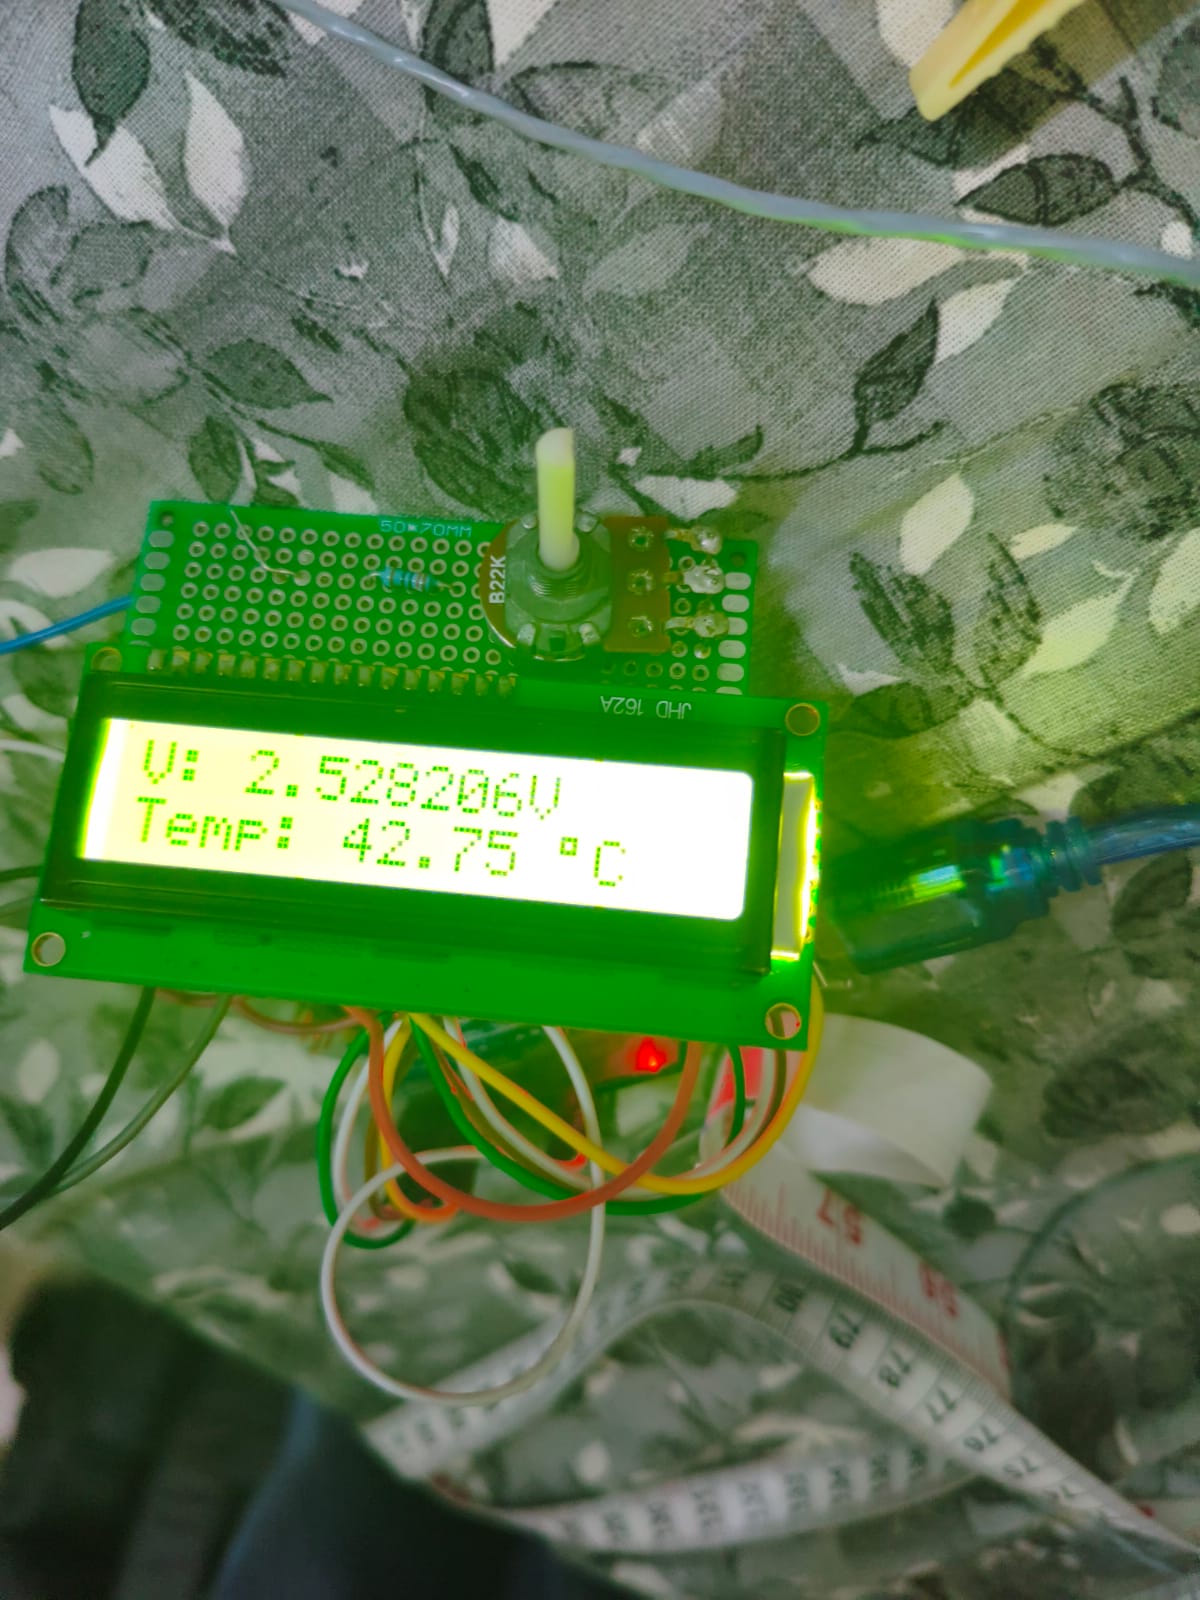
\includegraphics[width=\textwidth, height=10cm, keepaspectratio]{figs/Working-40.jpeg}
        \caption{Our reading ($40^\circ\text{C}$ range)}
    \end{subfigure}
    \hfill
    \begin{subfigure}{0.45\textwidth}
        \centering
        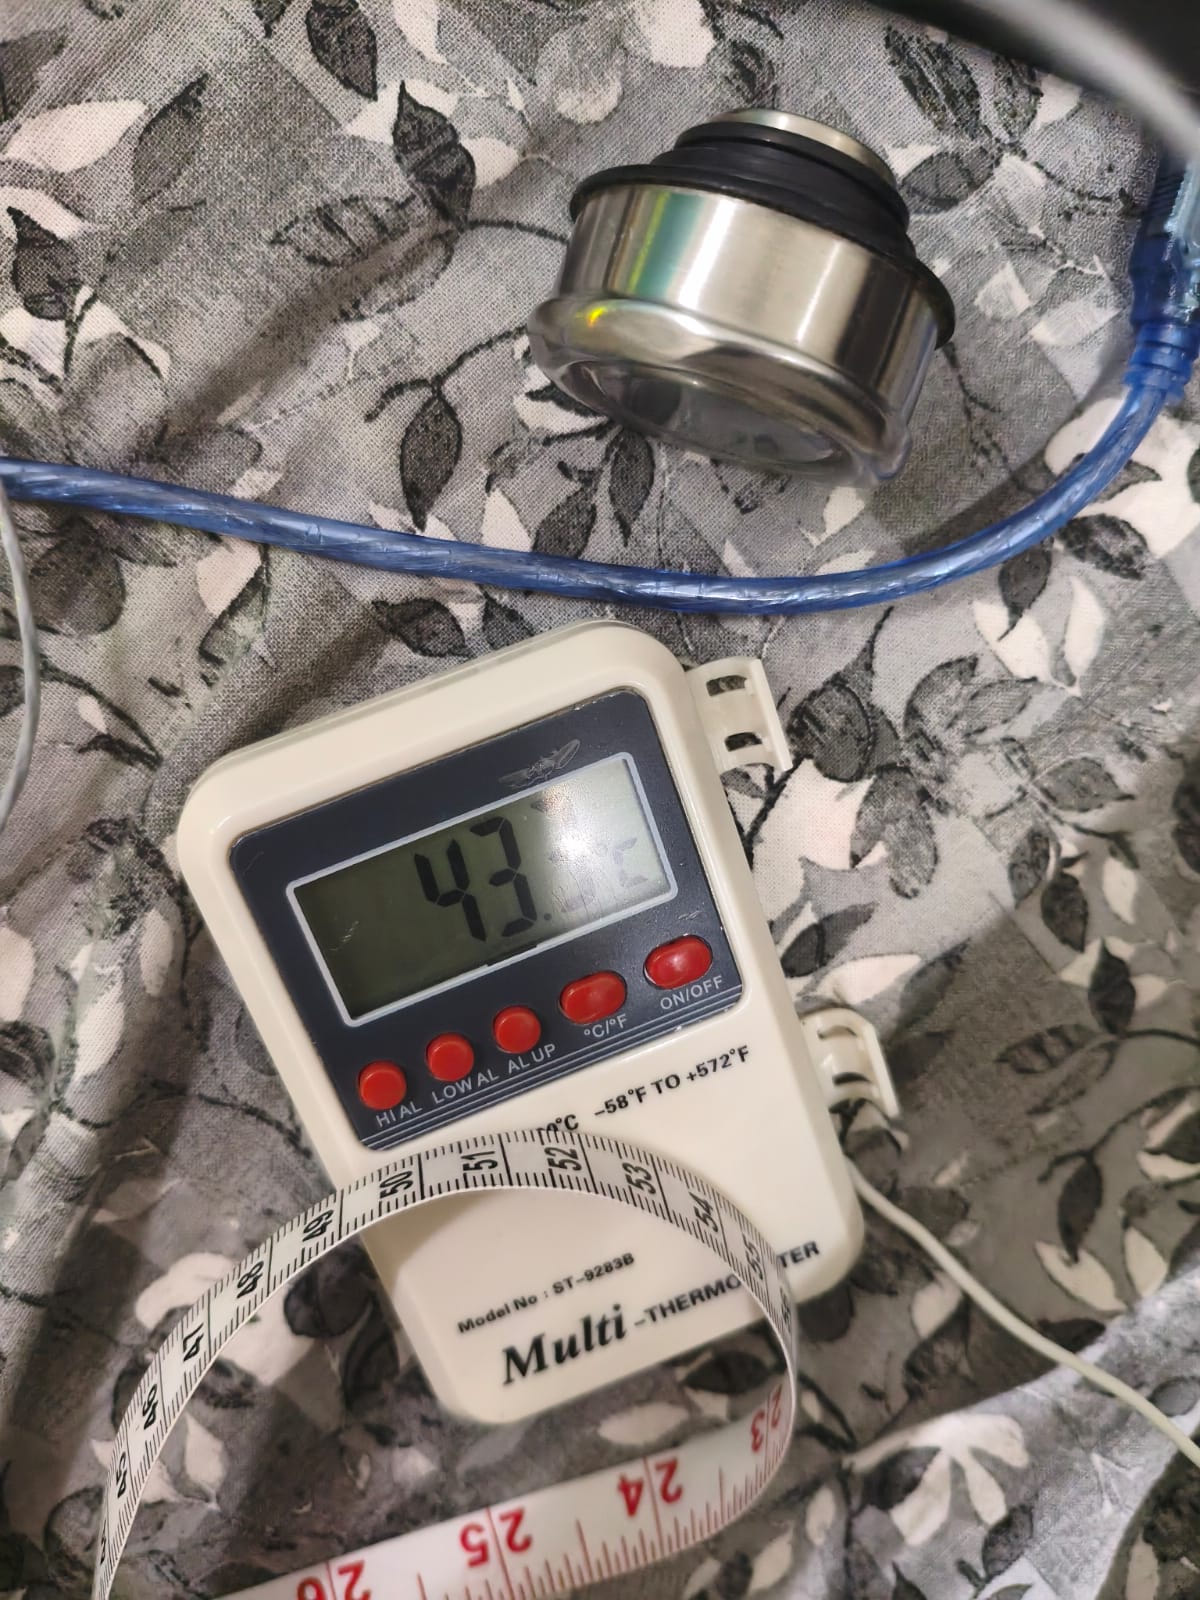
\includegraphics[width=\textwidth, height=10cm, keepaspectratio]{figs/Working-40_1.jpeg}
        \caption{Reference reading}
    \end{subfigure}
\end{figure}

\begin{figure}[H]
    \centering
    \begin{subfigure}{0.45\textwidth}
        \centering
        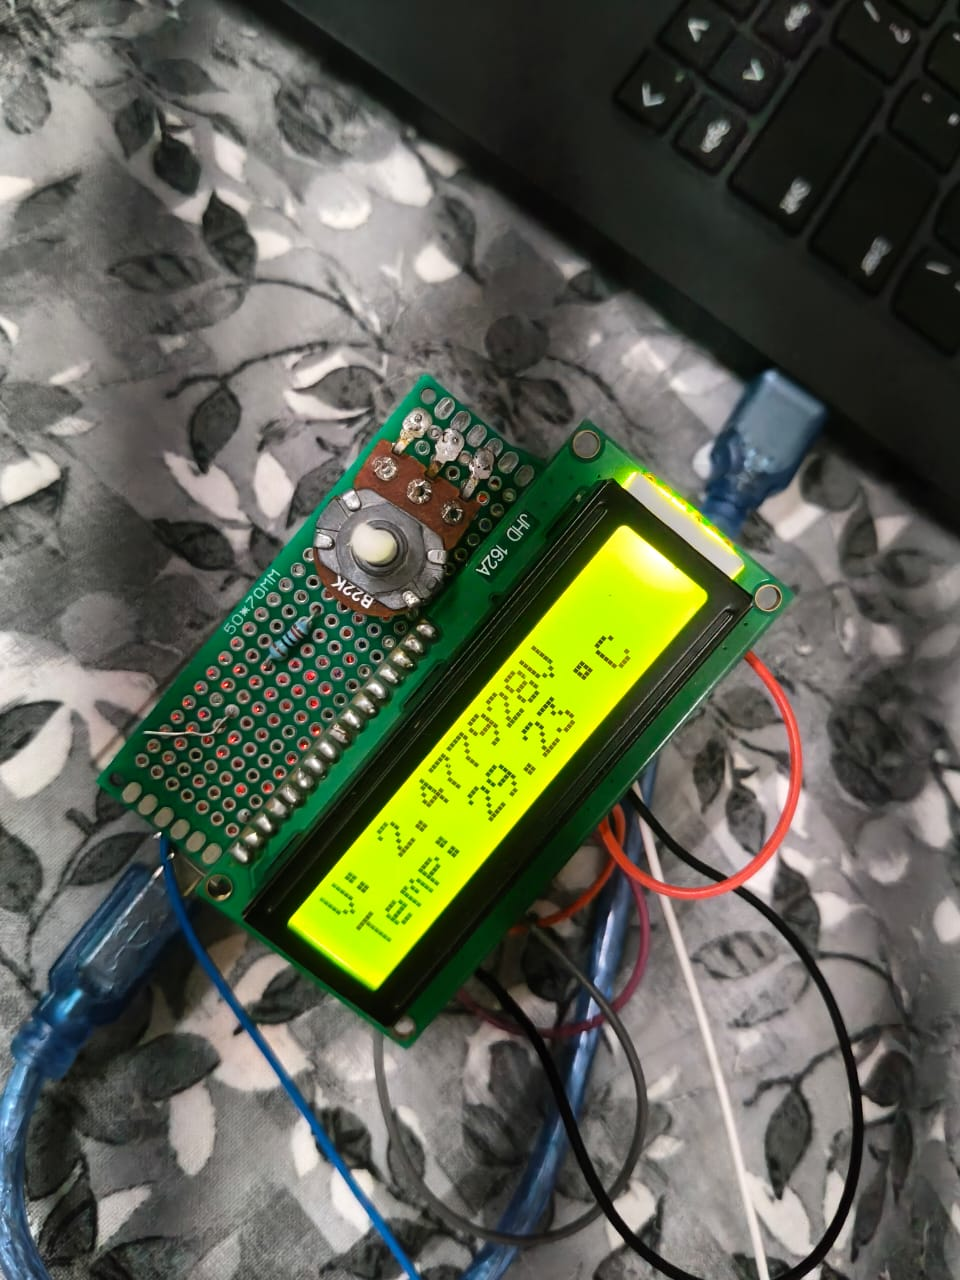
\includegraphics[width=\textwidth, height=10cm, keepaspectratio]{figs/Working-30.jpeg}
        \caption{Our reading ($30^\circ\text{C}$ range)}
    \end{subfigure}
    \hfill
    \begin{subfigure}{0.45\textwidth}
        \centering
        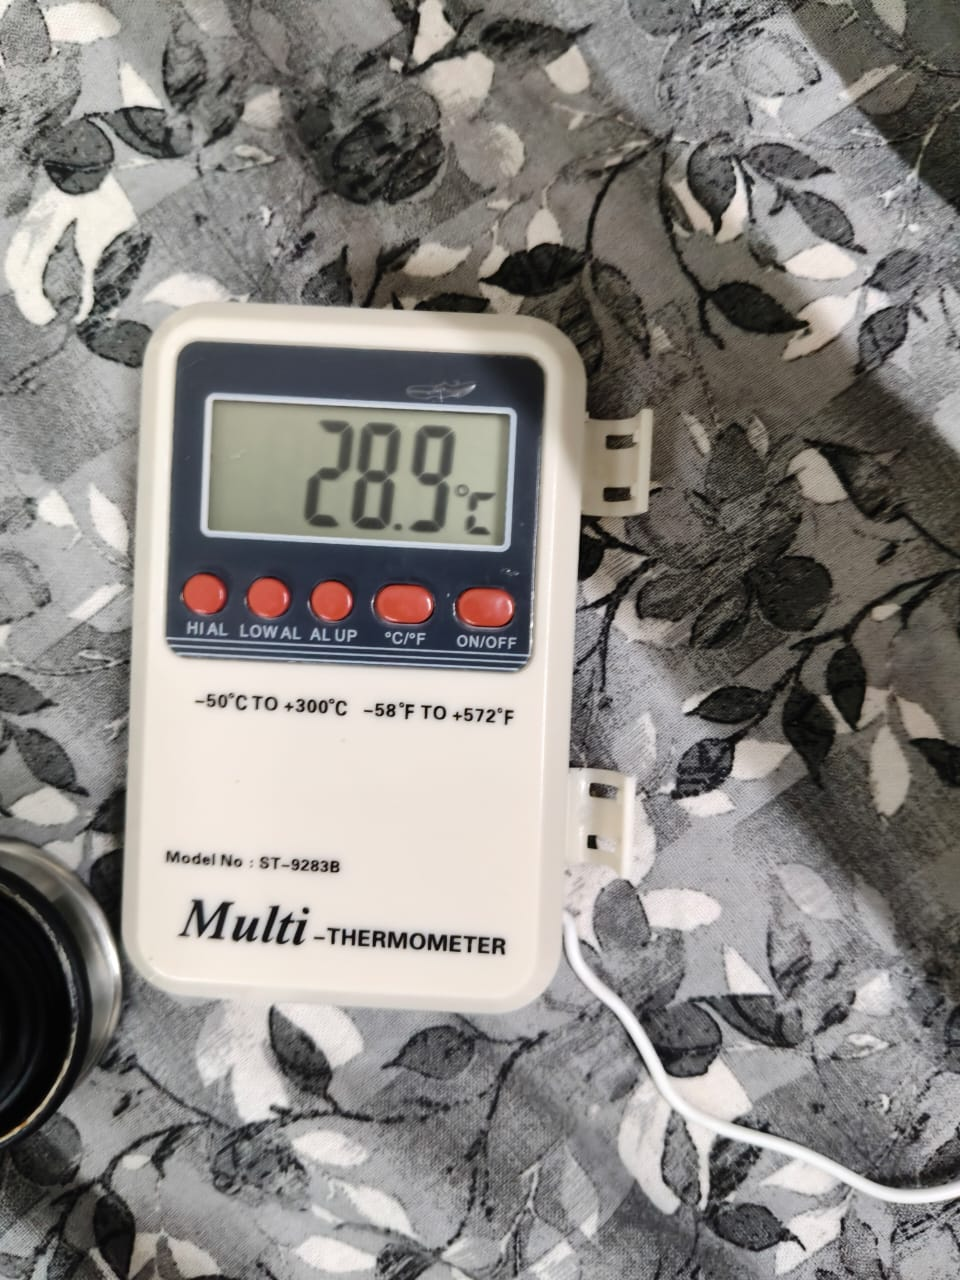
\includegraphics[width=\textwidth, height=10cm, keepaspectratio]{figs/Working-30_1.jpeg}
        \caption{Reference reading}
    \end{subfigure}
\end{figure}

\noindent{The calibration successfully reduced measurement deviations to within $0.4$--$1.5^\circ\text{C}$ across the entire operating range.}

\section*{Days 6 and 7 - CAD Modeling}
\noindent{The final stage involved CAD design for the physical enclosure. We designed a custom two-part casing in FreeCAD to house the Arduino Uno, soldered board, LCD screen, and potentiometer.} \\ \\

\noindent{We began by sketching the baseline perimeter and applying a pad extrusion:}
\begin{figure}[H]
    \centering
    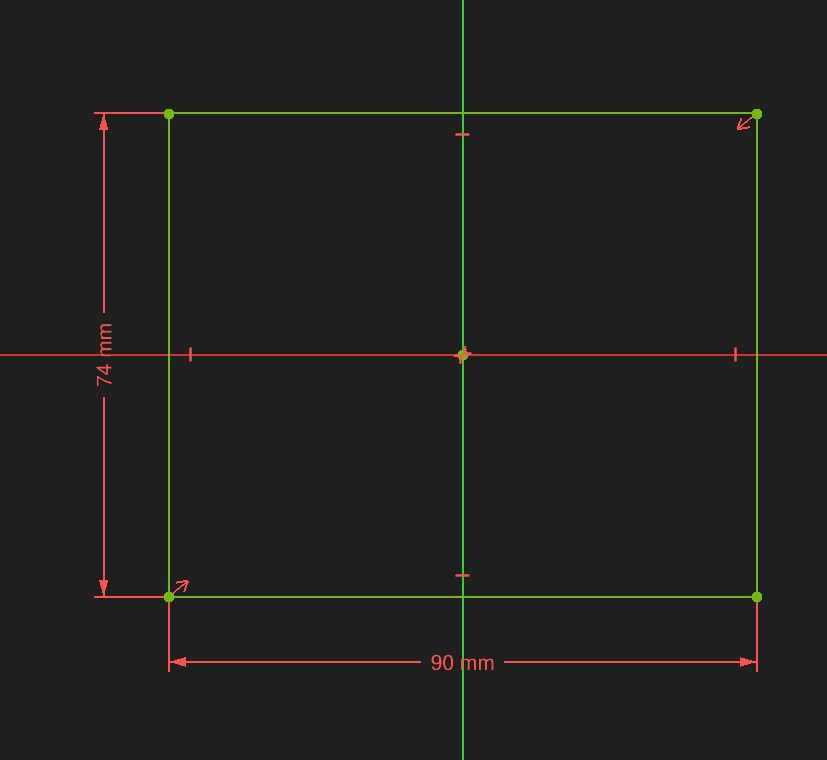
\includegraphics[width=0.5\linewidth]{figs/CAD_1.jpeg}
    \caption{Initial Sketch}
\end{figure}

\begin{figure}[H]
    \centering
    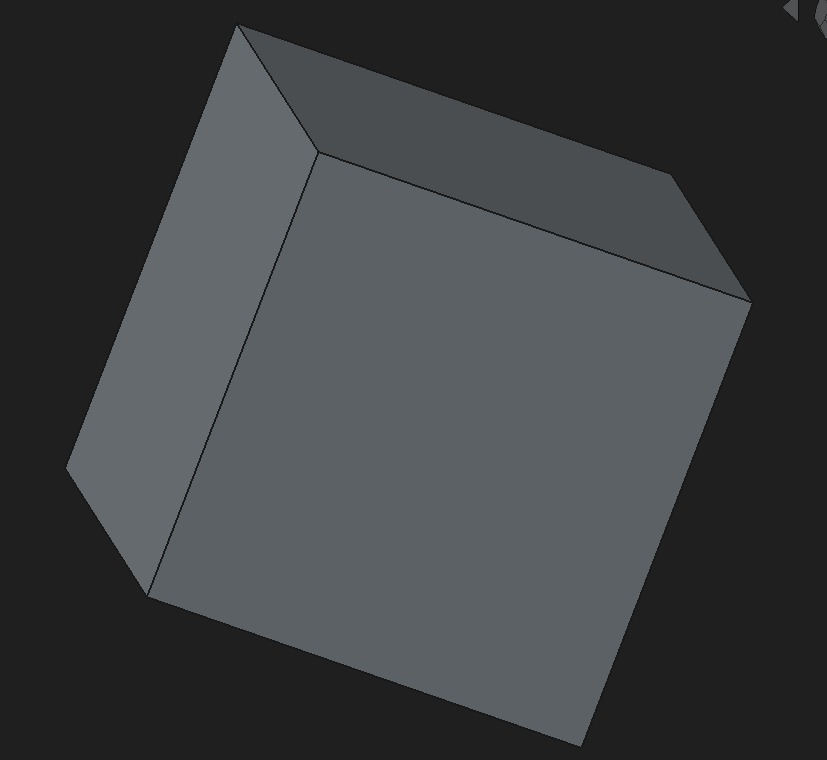
\includegraphics[width=0.5\linewidth]{figs/CAD_2.jpeg}
    \caption{Pad Extrusion}
\end{figure}

\noindent{Next, we hollowed out the interior body volume and designed mounting lips for the top lid:}
\begin{figure}[H]
    \centering
    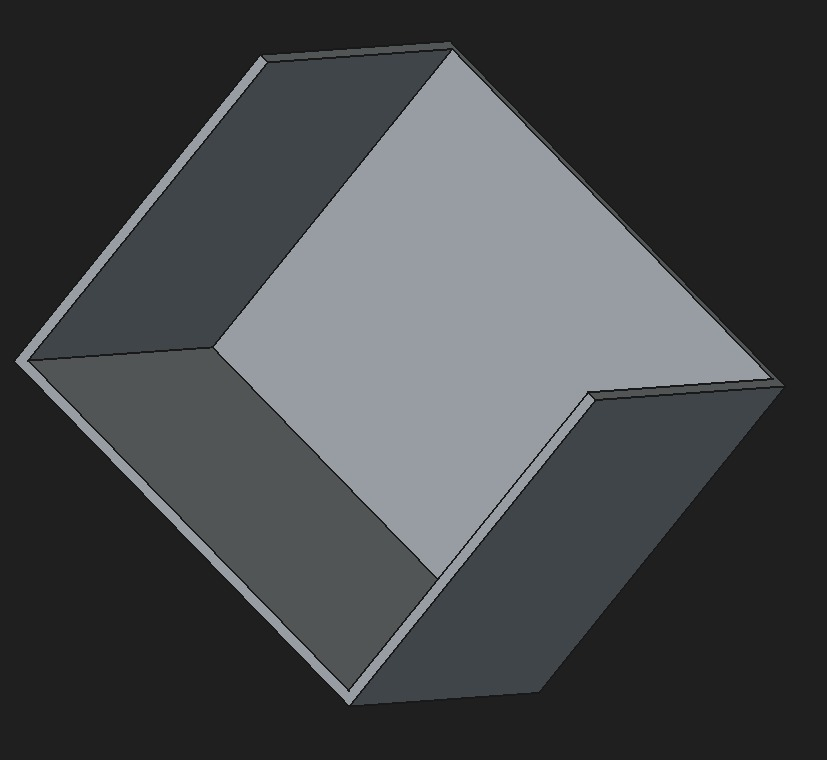
\includegraphics[width=0.5\linewidth]{figs/CAD_3.jpeg}
    \caption{Internal cavity hollow}
\end{figure}

\noindent{We then added standoffs and screw holes for securing the Arduino board:}
\begin{figure}[H]
    \centering
    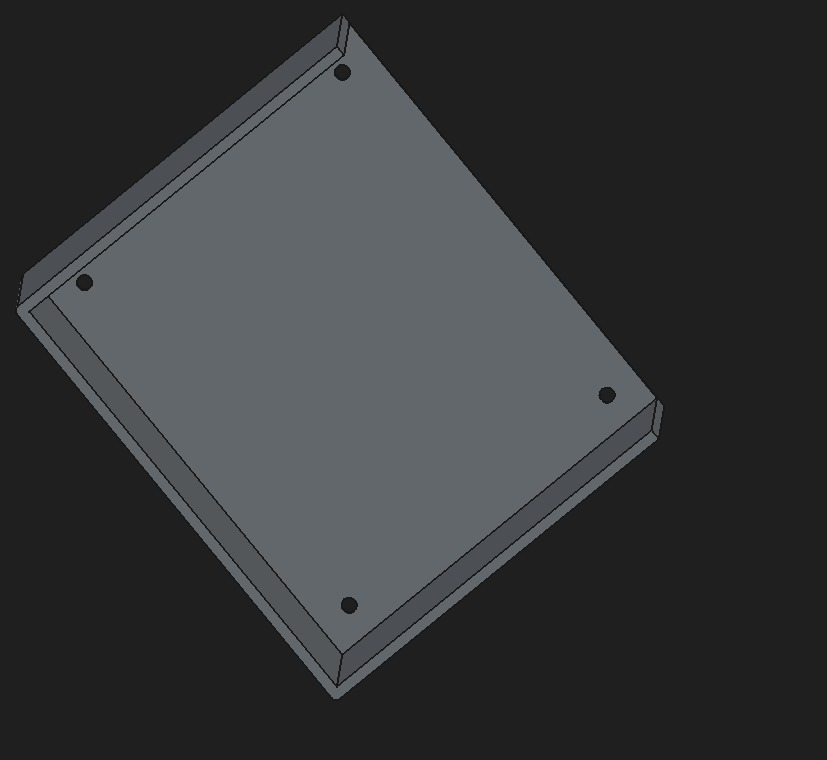
\includegraphics[width=0.5\linewidth]{figs/CAD_4.jpeg}
    \caption{Arduino mounting points}
\end{figure}

\noindent{Threaded mounting posts were added to fasten the top cover to the main body:}
\begin{figure}[H]
    \centering
    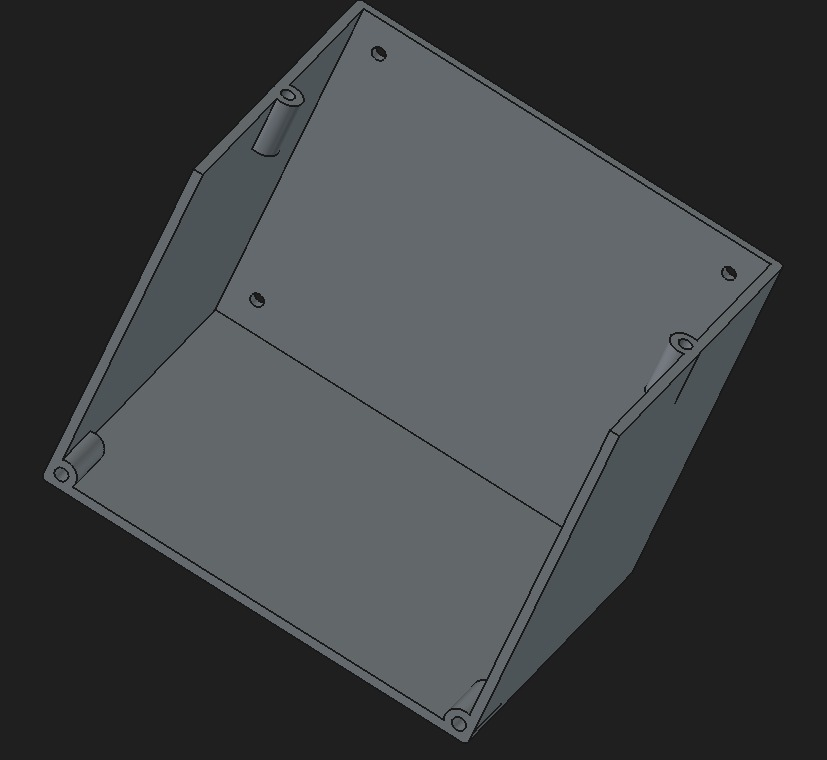
\includegraphics[width=0.5\linewidth]{figs/CAD_5.jpeg}
    \caption{Cover mounting standoffs}
\end{figure}

\noindent{Internal support rails and PCB mounting pegs were added next:}
\begin{figure}[H]
    \centering
    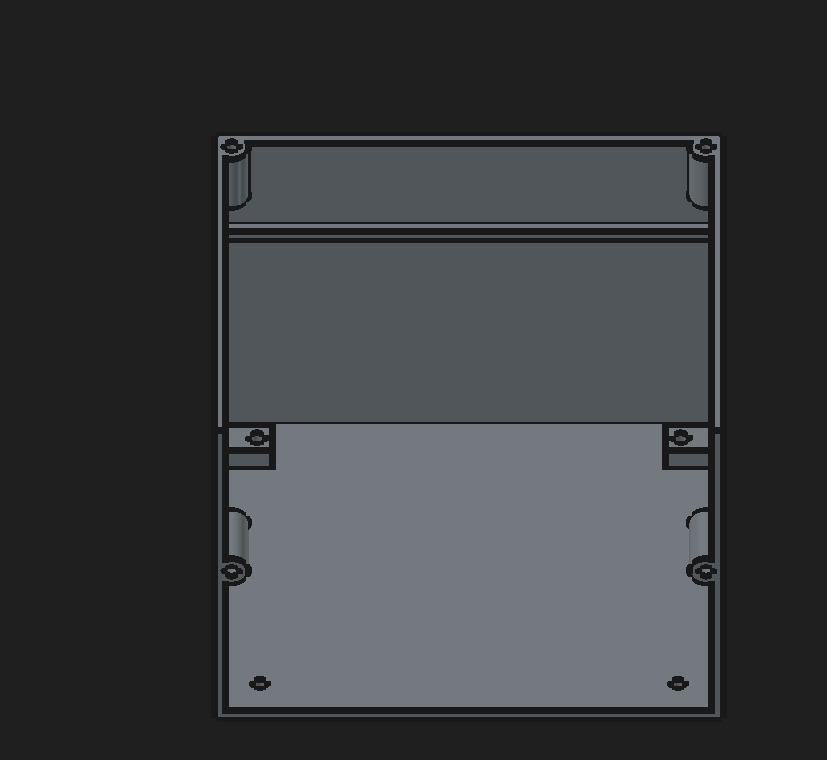
\includegraphics[width=0.5\linewidth]{figs/CAD_6.jpeg}
    \caption{PCB support structure}
\end{figure}

\noindent{A cable spool feature was incorporated to manage excess PT100 lead wire length:}
\begin{figure}[H]
    \centering
    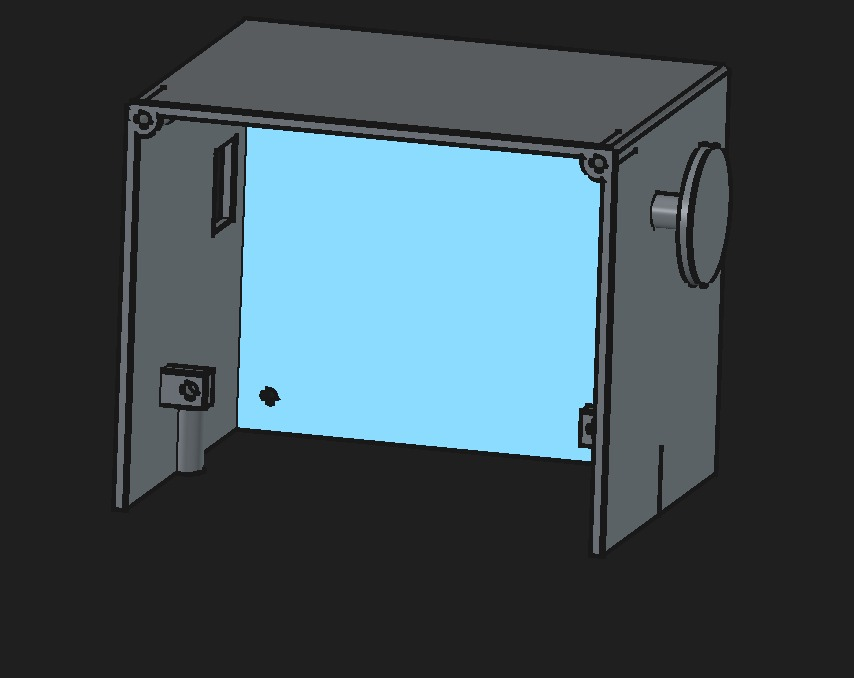
\includegraphics[width=0.5\linewidth]{figs/CAD_7.jpeg}
    \caption{Integrated cable spool}
\end{figure}

\noindent{We then added an external storage holder clip for securing the PT100 probe:}
\begin{figure}[H]
    \centering
    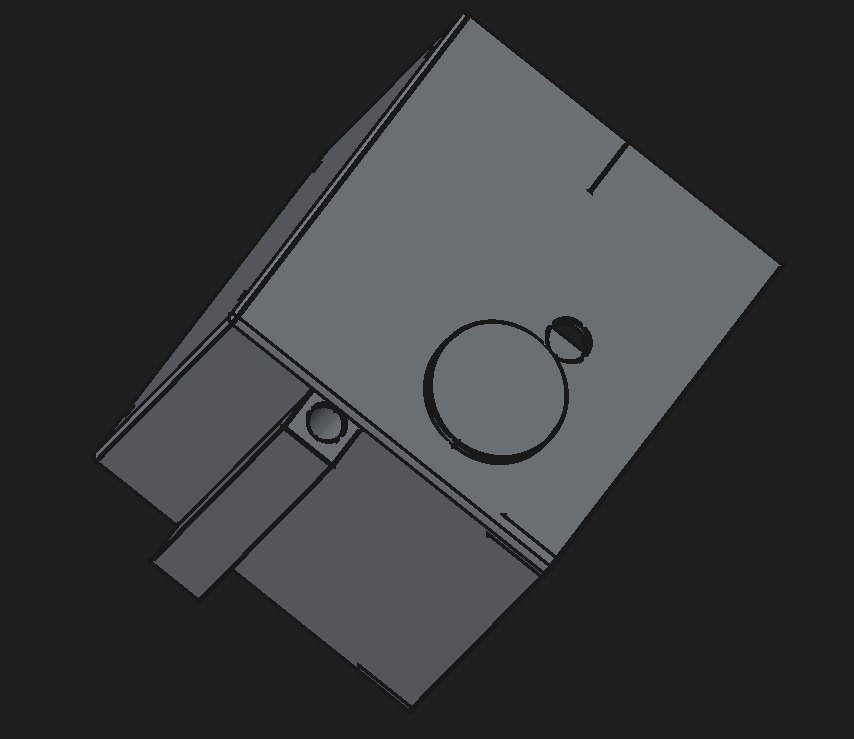
\includegraphics[width=0.5\linewidth]{figs/CAD_8.jpeg}
    \caption{PT100 probe holster}
\end{figure}

\noindent{Finally, cutouts for the 16x2 LCD display screen and contrast adjustment potentiometer knob were added to the lid, completing the 3D enclosure model:}
\begin{figure}[H]
    \centering
    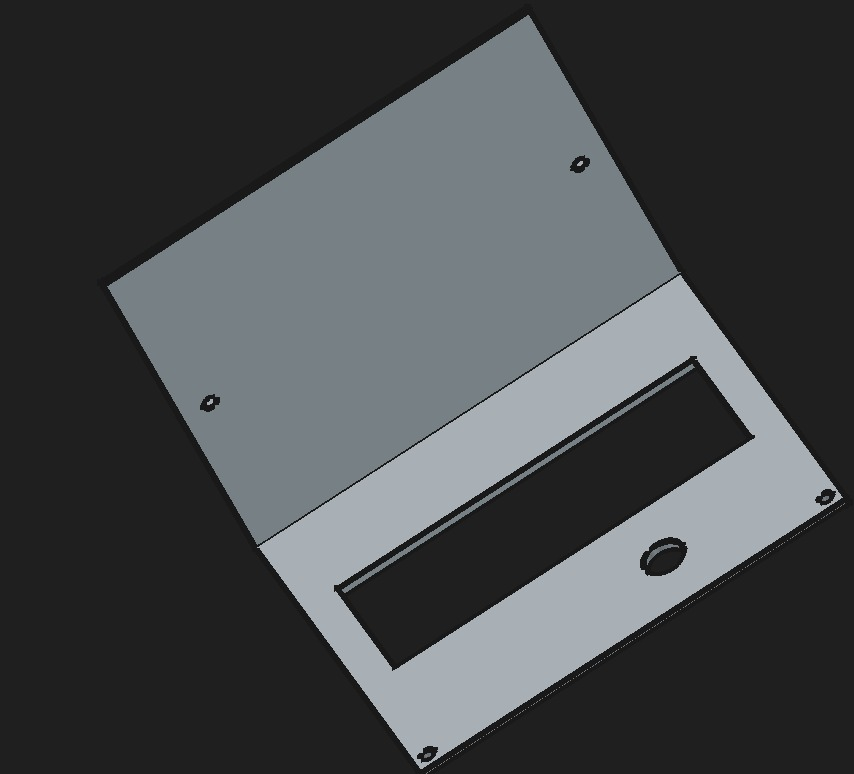
\includegraphics[width=0.5\linewidth]{figs/CAD_9.jpeg}
    \caption{Final assembled CAD model}
\end{figure}
\section*{Learnings}
\begin{itemize}
    \item Gained practical troubleshooting experience by systematically isolating individual hardware components.
    \item Learned the necessity of custom Least Squares (LSQ) regression when working with non-ideal component tolerances and differing supply voltages ($V_{\text{cc}} = 5.08\,\text{V}$) Relying on theoretical or paper models introduced systematic offsets, whereas collecting an overdetermined empirical calibration dataset ($V, T$) directly mapped out lead wire resistance and non-linear PT100 behavior.
    \item Learned how mechanical constraints dictate electrical component layout. Pivoting from a sliding-lid mechanism to a screwed-down enclosure demonstrated the importance of evaluating 3D-printing tolerances, structural rigidity, and ease of assembly during early CAD prototyping.
    \item Improved project management and agile problem-solving under a hard deadline. Iterative brainstorming allowed us to quickly adapt, re-calibrate after wire re-soldering, and successfully optimize model precision to within $0.4$--$1.5^\circ\text{C}$.
\end{itemize}
\section*{Future Work}
We wish to explore machine learning data augmentation and regularization techniques (e.g., Gaussian noise injection or Mixup interpolation) to train higher-capacity regression models if deployed across non-linear sensor networks.
\end{document}
